\documentclass[12pt]{report}
\usepackage{amsmath}
\usepackage{amsfonts}
\usepackage{amssymb}
\usepackage{textcomp}
\usepackage{graphicx}
\usepackage{float}
\usepackage{hyperref}
\usepackage[a4paper, margin = 1in]{geometry}

\usepackage[draft]{todonotes}


%Commands used in text, edit here and the document will populate with correct value.
\newcommand{\projectName}{CEPAD }
\newcommand{\payLoadMass}{3.352Kgs }

\makeatletter
\newcommand*\bigcdot{\mathpalette\bigcdot@{.5}}
\newcommand*\bigcdot@[2]{\mathbin{\vcenter{\hbox{\scalebox{#2}{$\m@th#1\bullet$}}}}}
\makeatother

%*******************************TITLE PAGE*******************************%

\title{Development of a Close Quarter Collision Protected Aerial Drone}
\author{Angus Steele} 

\begin{document}
\section{Horizontal Control}
This section describes the horizontal controller. This system is responsible for controlling the craft's North and East position in the earth frame, to do this the controller's most inner loop commands the pitch and roll rates of the craft. The narrow, confined spaces in which the craft must fly means it is very important for the horizontal controller to respond quickly to commands and disturbances. The limited space also limits the amount of allowed overshoot, requiring a well damped final system. While the system should be fast, it must stay within it's thrust limits as to not affect the other controllers. The controller will need to be able reject disturbances caused by wind, sensor offsets and unbalanced rotors. To handles these disturbances and other, the system will require an integrator in the controller. The integrator should be fast enough as to ensure the system stays within it's narrow, permissible flight region, even during disturbances.

The horizontal controller is designed as two sets of four cascaded control loops, one set for roll and one set for pitch. The most inner loop controls either the roll or pitch rate of the craft by commanding the virtual actuators $\delta_\phi$ and $\delta_\theta$ respectively. The desired angular rates are in turn commanded by the tilt angle controller. The tilt angle controller is responsible for converting desired translational accelerations into desired roll and pitch angles. These acceleration setpoints are commanded by the linear velocity controller which receives it's setpoint from the most outer global position controller. The global position controller will receive it's setpoint from the waypoint generation method described in a proceeding section. This section begins by deriving the plant dynamics for roll and pitch.

\subsection{Roll and Pitch Rate Dynamics}
The roll and pitch acceleration dynamics can be derived using Newton mechanics at near hover conditions and the craft's inertia around the X-axis ($I_{xx}$) and the Y-axis ($I_{yy}$) respectively, the result is shown in \eqref{EQ_RollNewton} and \eqref{EQ_PitchNewton}.

\begin{equation}
\label{EQ_RollNewton}
\dot{p} = \dfrac{L}{I_{xx}}
\end{equation}

\begin{equation}
\label{EQ_PitchNewton}
\dot{q} = \dfrac{M}{I_{yy}}
\end{equation}

The rotors introduce an additional timing delay into the dynamics, as shown in \eqref{EQ_MotorDelay}. The state space equation for both systems can be derived using the current angular rates ($p$ \& $q$) and the current angular moments ($L$ \& $M$) as the system states. The state space representation for roll is shown in \eqref{EQ_RollStateSpace1} and \eqref{EQ_RollStateSpace2}. The transfer function for roll acceleration can subsequently be calculated from the state space representation. Integrating the result produces the transfer function for roll rate as shown in \eqref{EQ_RollTF}. The same approach is followed for deriving the pitch rate dynamics shown in \ref{EQ_PitchTF}.

\begin{eqnarray}
\begin{bmatrix} \dot{L} \\ \dot{p}	\end{bmatrix}&=&\begin{bmatrix}\frac{1}{\tau}\ \ \ \ \ 0\\\frac{1}{I_{xx}} \ \ \ 0 \end{bmatrix} \begin{bmatrix} L \\ p \end{bmatrix} + \begin{bmatrix}\frac{1}{\tau}\\ 0 \end{bmatrix} \delta_\phi\label{EQ_RollStateSpace1}\\\label{EQ_RollStateSpace11} 
y &=& \begin{bmatrix} 0 \ \ \ \ 1 \end{bmatrix} \begin{bmatrix} L \\ p \end{bmatrix} \label{EQ_RollStateSpace2}\\
G(s)_{roll} &=& \frac{\frac{1}{\tau I_{xx}}}{s (s + \frac{1}{\tau})}\label{EQ_RollTF}\\
G(s)_{pitch} &=& \frac{\frac{1}{\tau I_{yy}}}{s (s + \frac{1}{\tau})}\label{EQ_PitchTF}
\end{eqnarray}

The roll and pitch plants both have a naturally occurring integrator, an open loop pole at $-\dfrac{1}{\tau}$ and no naturally occurring zeros. As shown, the plant gain is inversely proportional to the specific axis inertia. The design of the craft creates a smaller pitching plant gain than rolling plant gain. The design however, gives the pitching moment a longer torque arm, creating a larger actuation torque.

\subsection{Roll and Pitch Rate Controllers}
The roll and pitch rate controllers are the most inner loops of the horizontal controller and they command the $\delta_\phi$ and $\delta_\theta$ virtual actuators respectively. As the most inner controllers the outer loops of the horizontal controller are limited by the response and bandwidth of this system. Both these systems should then utilise as much bandwidth as the physical motor-rotor system allows. Section \ref{SSECT_Disturbances} describes some of the expected disturbances where induced moments can be caused in multiple scenarios. Including being in near proximity with a wall or having unbalanced rotor pairs. The final system must track a set point with zero steady state error. To meet the horizontal controller's requirement of fast disturbance rejection, the roll and pitch rate controllers, as the fastest controllers, should include an integrator. 

The integrator will slow the system down, which can be subsequently sped up with a lead compensator. However, the final commanded motor thrusts must be validated against the limits provided in Table \ref{tab:HeadRoomPercentages}. The final controller architecture is shown in Figure \ref{IM_RollPitchRateController}. The controller gain values must be chosen such that the inner rate system is robust to unmodelled errors and have a sufficient gain and phase margin.

\begin{figure}[H]
	\centering
	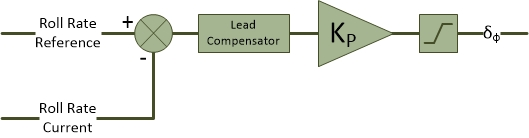
\includegraphics[height = 3.3cm]{../References/Diagrams/RollRateController.jpg}
	\caption{Roll and Pitch Rate Controller Design}
	\label{IM_RollPitchRateController}
\end{figure}	

First, the dynamic response of the controlled roll system is evaluated using the root locus shown in Figure \ref{IM_RollRateControlRoot}. To maintain good damping, the two dominant poles are kept close to the imaginary axis and have a final damping ratio of $0.9$. Where the placement of the slower zero dictates how much influence the integrator can have on the system. \todo[inline]{Making reference to how the zero's location is the ratio of Ki/Kp, but when I say it like this I get worried it might not be completely accurate?}

\begin{figure}[H]
	\centering
	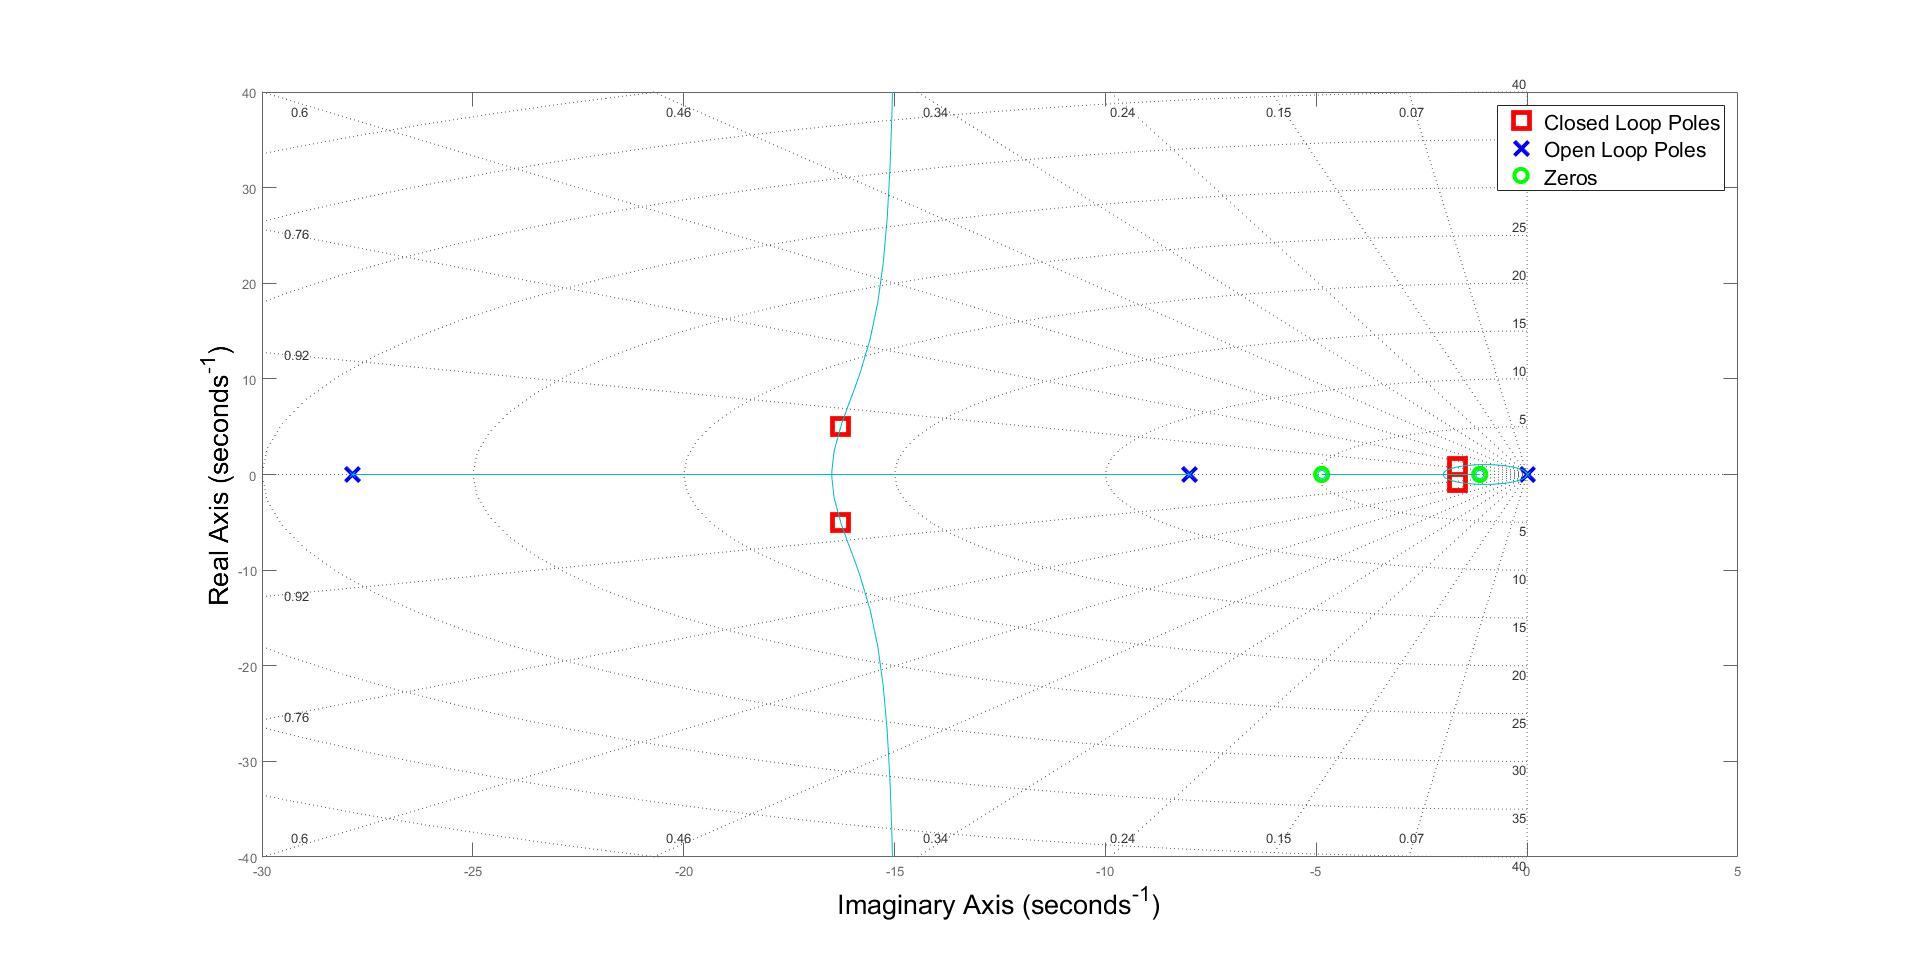
\includegraphics[height = 8cm]{../Design/Matlab/Controllers/roll_rate_root.jpg}
	\caption{Roll Rate Controller -  Root Locus}
	\label{IM_RollRateControlRoot}
\end{figure}

The frequency response of the roll system is then investigated using the Bode plot shown in Figure \ref{IM_RollRateControlBode}. Unity feedback is compared against the chosen controller. The high natural gain of the rolling system gives unity feedback a very fast result with too much bandwidth for the physical system to match. There is also an insufficient phase margin of $25$\textdegree\,in the system and no offset disturbance rejection. The controller adds an integrator to reject disturbances, this however reduces phase even more and slows the system. The lead compensator is then used to increase the phase and bandwidth and reach a final phase margin of $80.6$\textdegree\,with a crossover frequency of $4.75$\,rad/s.

\begin{figure}[H]
	\centering
	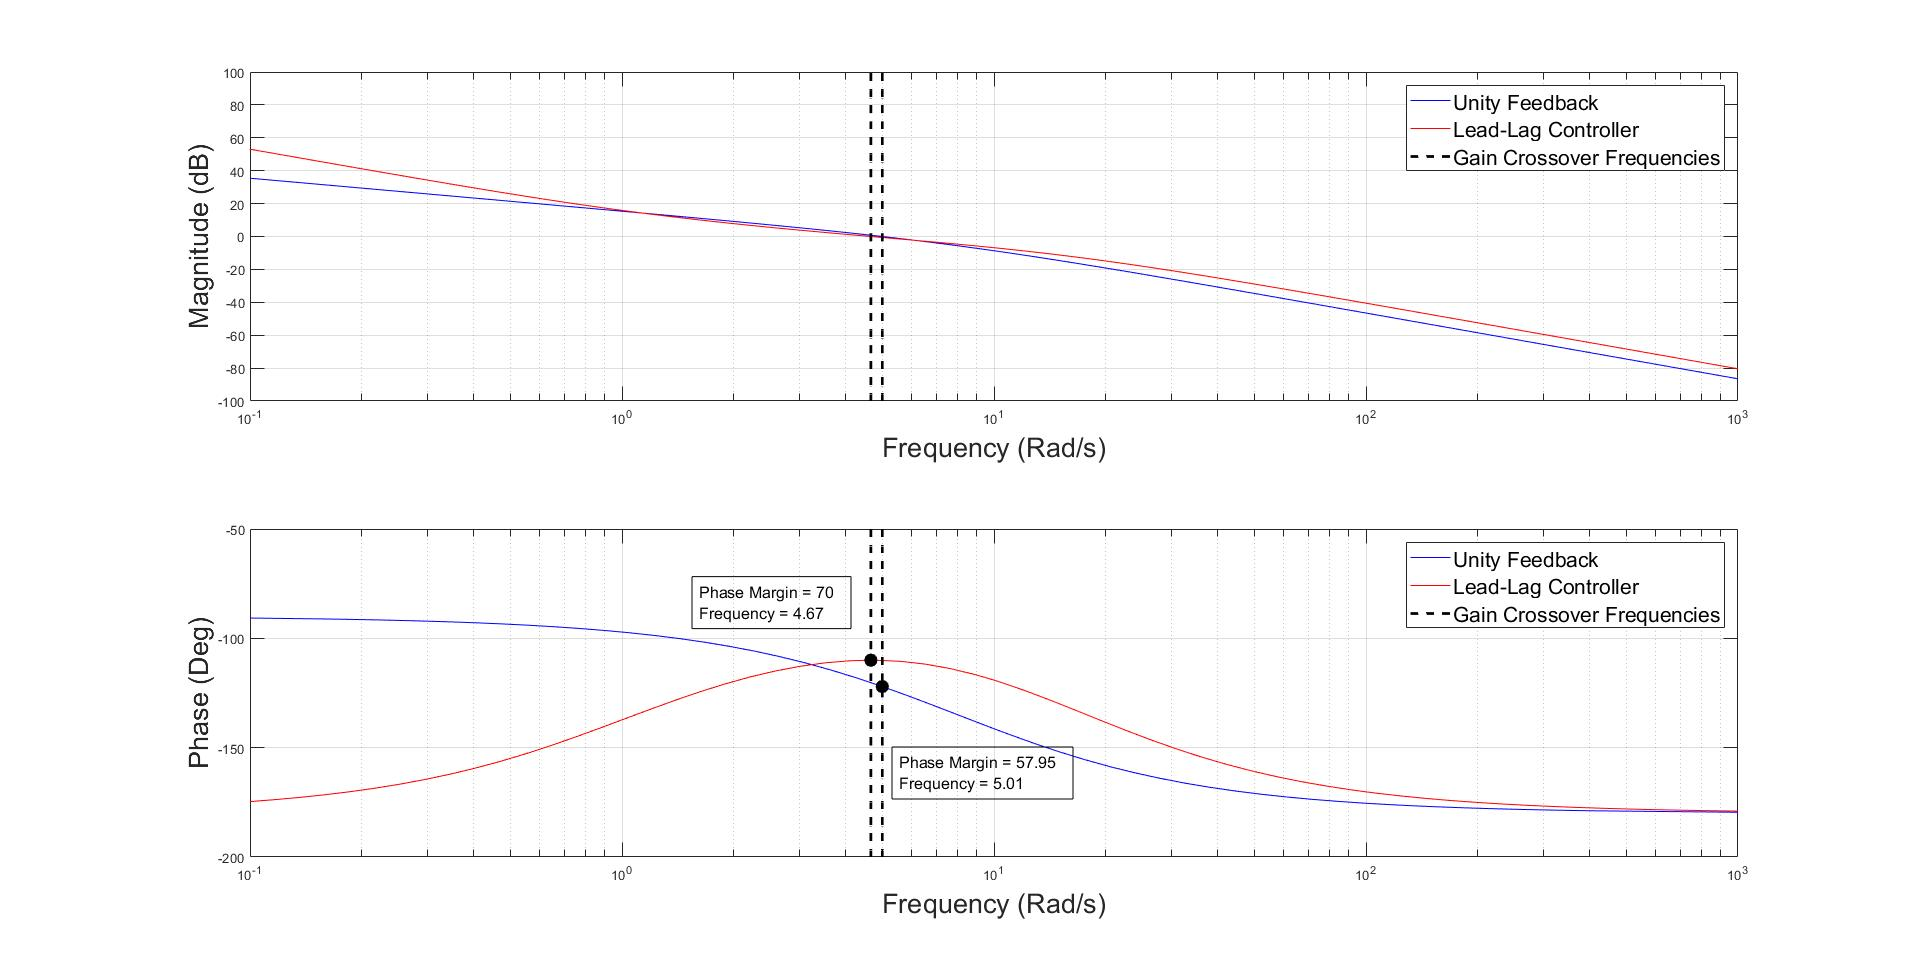
\includegraphics[height = 8cm]{../Design/Matlab/Controllers/roll_rate_bode.jpg}
	\caption{Roll Rate Controller -  Bode Plot}
	\label{IM_RollRateControlBode}
\end{figure}

Next the pitch rate system is evaluated. The loci and closed loop poles of the controlled pitch system can be shown to be similar to the roll system. However, the pitching plant is naturally slower and has less gain than the rolling system. The pitch rate controller is thus required to have more gain than the roll rate controller. The Bode plot shown in Figure \ref{IM_PitchRateControlBode} is used to evaluate the frequency response of the pitch rate system. Unity feedback is compared against the implemented Lead-Lag controller. As shown the natural system with unity feedback produces a much lower crossover bandwidth than the natural roll system. As with the roll rate controller, the integrator included in the controller reduces phase and bandwidth in the system but also enables disturbance rejection. To speed up the system, a similarly placed lead compensator is used. This increases the phase and bandwidth to reach a final phase margin of $82.2$\textdegree\,with a crossover frequency of $4.72$\,rad/s.

\begin{figure}[H]
	\centering
	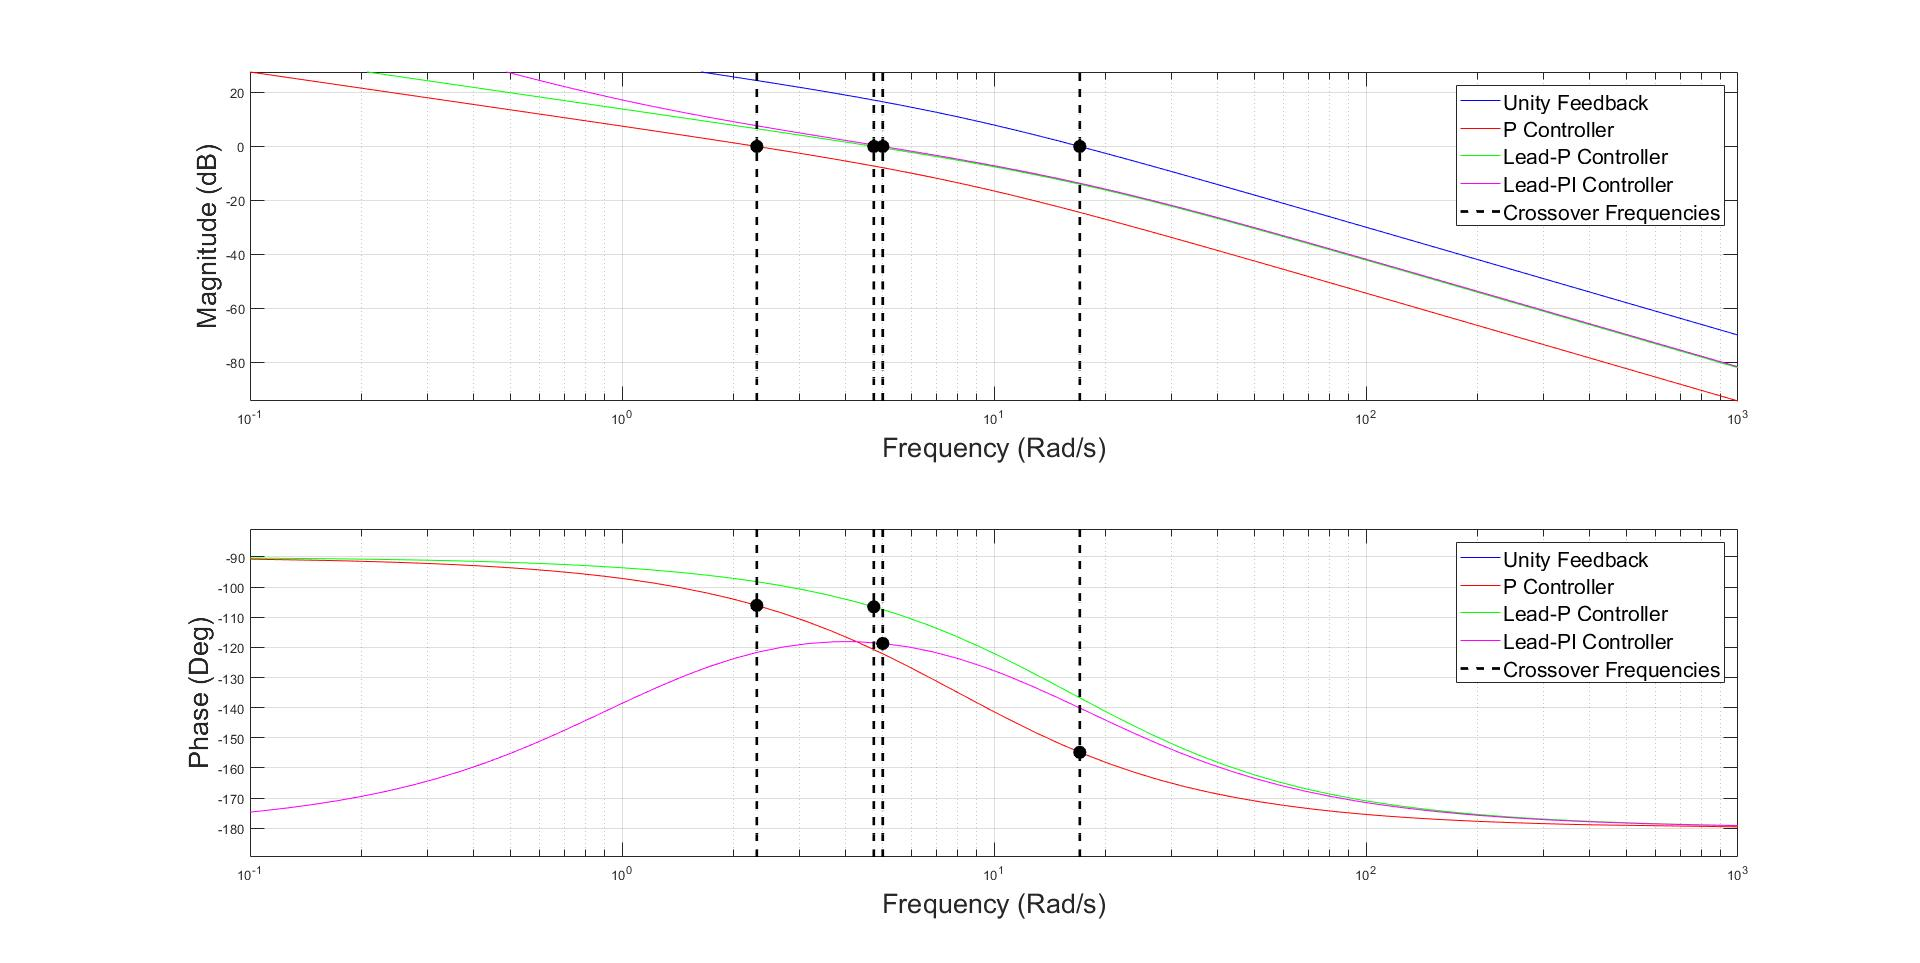
\includegraphics[height = 8cm]{../Design/Matlab/Controllers/pitch_rate_bode.jpg}
	\caption{Pitch Rate Controller -  Bode Plot}
	\label{IM_PitchRateControlBode}
\end{figure}


\subsubsection{Roll and Pitch Rate Controller Discussion}
The dynamic responses of the roll and pitch rate systems is shown to be robust, damped and they both utilise the full bandwidth allowed by the system characteristics. The integrator term in both controllers will ensure that the rate loop can handle steady state disturbances. To stop integrator wind up however, the controllers include a saturation on the integral term. Although both systems have the same controller architecture, the physical design of the craft means the roll system will have a larger plant gain. It is desired that the roll and pitch rate systems have similar closed loop responses which means the pitch rate controller needs to have increased gain compared to the roll rate controller. This unfortunately leaves the roll rate controller to be more susceptible to disturbances. The flight strategy should take this into consideration and negate rolling disturbances as much as possible.

This characteristic can be shown in the time domain using step responses and the maximum impulse required of the motors. To enable a comparison between the systems, the step response of both the roll and pitch rate system is shown in Figure \ref{IM_PitchRateStep}. To simulate a disturbance, a $0.05$\,Nm loss in torque is applied to the roll system at $5$\,s. The pitching system experiences a disturbance of $0.2$\,Nm. Both disturbances are calculated and equivalent to two rotors, on the same side, instantaneously losing $0.25$\,N of thrust.

\begin{figure}[H]
	\centering
	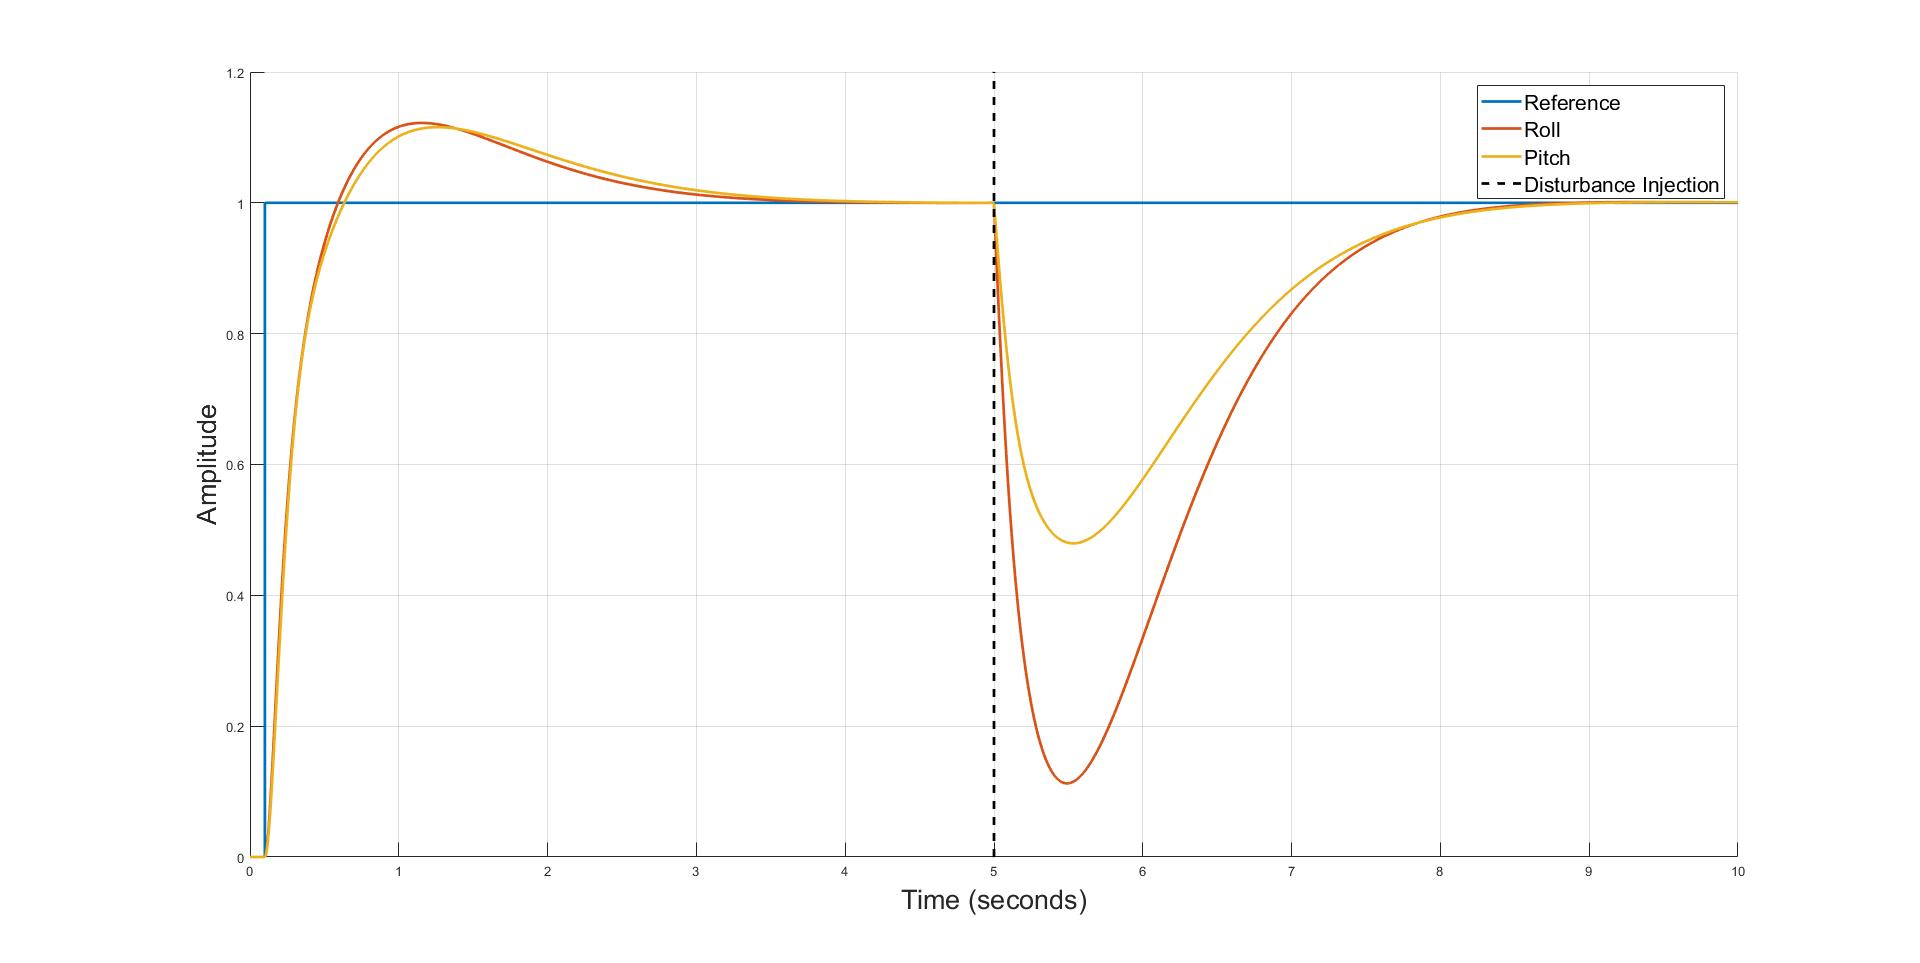
\includegraphics[height = 8cm]{../Design/Matlab/Controllers/roll_pitch_rate_step.jpg}
	\caption{Pitch Rate Controller -  Step Responses}
	\label{IM_PitchRateStep}
\end{figure}

Both the roll and pitch closed loop systems have similar transient responses. The pitch rise time of $0.33$\,s is very similar to the roll rise time of $0.32$\,s. The pitch $5$\,\% settling time is measured at $2.2$\,s which is also very close to the rolling settling time of $2.1$\,s. Both systems are similarly damped and have overshoot of $12$\,\%. Limiting the integral term can reduce the overshoot however, this will also limit the disturbance rejection capabilities of the system. Both the roll and pitch systems handle the disturbance successfully and settle back within $5$\,\% of the setpoint in $2.6$\,s. As expected, the roll system has more difficulty handling the disturbance.

The commands sent to the rotors during the roll step are shown in Figure \ref{IM_RollRateImpulse} with a maximum commanded thrust of $0.49$\,N. Similarly, the pitching motor outputs are shown, in Figure \ref{IM_PitchRateImpulse}, to have a maximum thrust of $0.69$\,N.

\begin{figure}[H]
	\centering
	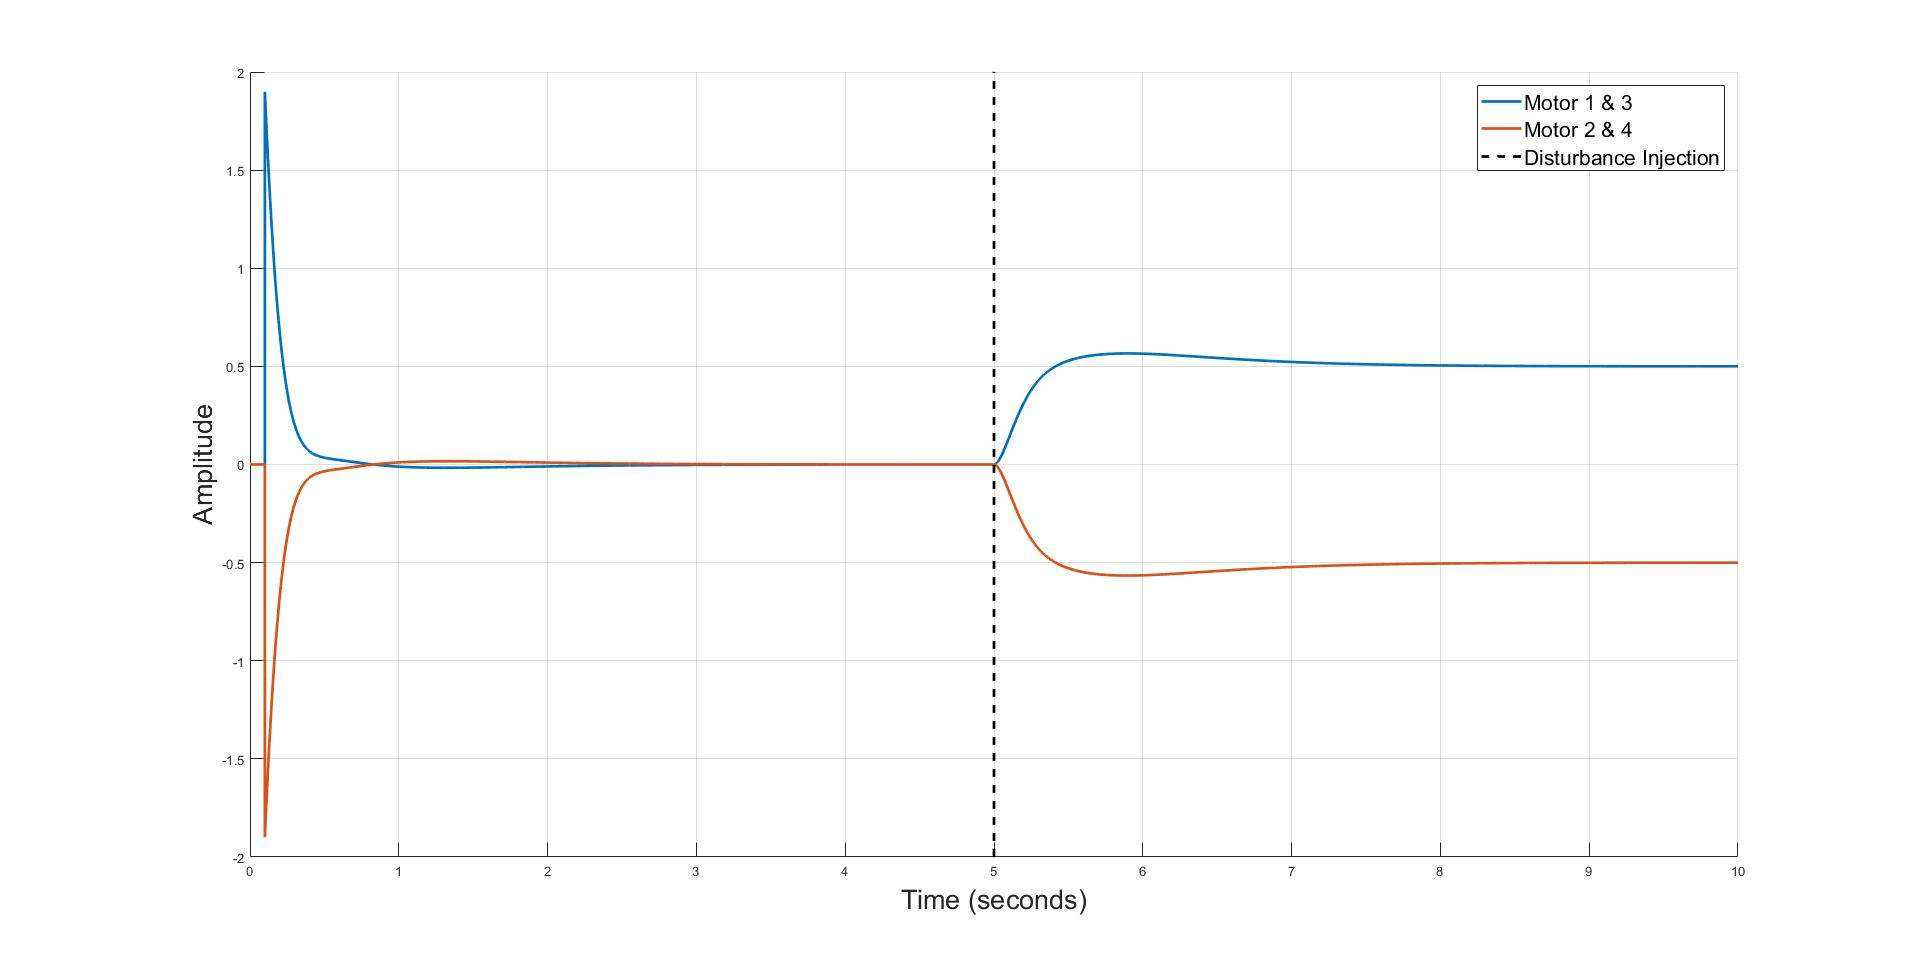
\includegraphics[height = 8cm]{../Design/Matlab/Controllers/roll_rate_impulse.jpg}
	\caption{Roll Rate Controller -  Motor Commands}
	\label{IM_RollRateImpulse}
\end{figure}

\begin{figure}[H]
	\centering
	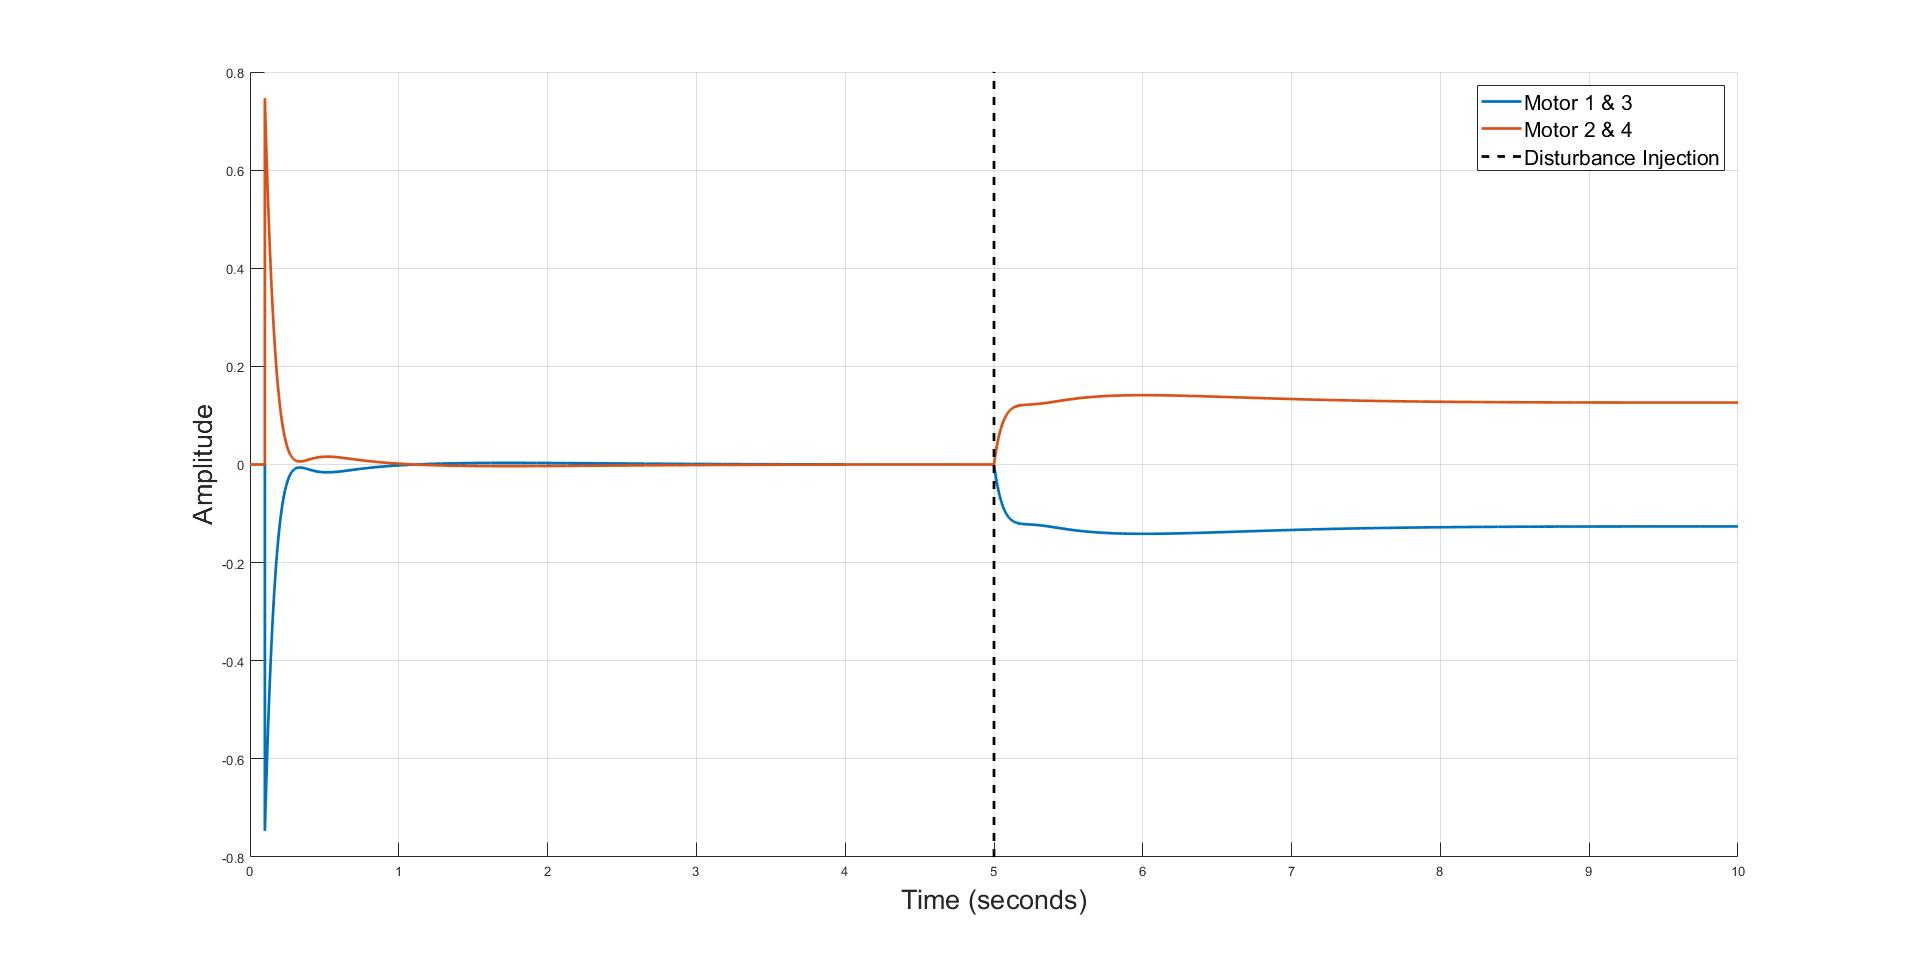
\includegraphics[height = 8cm]{../Design/Matlab/Controllers/pitch_rate_impulse.jpg}
	\caption{Pitch Rate Controller -  Motor Commands}
	\label{IM_PitchRateImpulse}
\end{figure}

Intuitively it can be strange that the pitching step response produces larger motor outputs than the rolling step. The longer pitch actuator arm would lead one to believe that the pitch system will command lower values of thrust. This is only true for a similar moment. The differing inertias entails that for a rate step response the rolling plant will produce a lower moment impulse as compared to the pitching system. To quantify the effect of the arm length versus the effect of the inertias both can be represented as ratios. The ratio between the roll and pitch arm lengths is $3.73$ where the ratio between the inertias is $6.76$. Therefore the pitch system has to work, ratio metrically, $1.81$ times harder than the rolling system resulting in larger motor thrust outputs.

\subsection{Tilt Angle Controller}
The tilt angle controller is responsible for controlling the desired roll and pitch angles of the craft. The controller does this by commanding angular rates it calculates from a translational acceleration reference in the earth frame. Using the current angular position, this earth frame acceleration reference is converted to the body frame and used to calculate the error in angular positions for roll and pitch. This error is then fed through a Proportional gain. This section makes reference to Figure \ref{IM_TiltAngleController} and begins by explaining the method used for converting the acceleration reference into desired angular rates.

\begin{figure}[H]
	\centering
	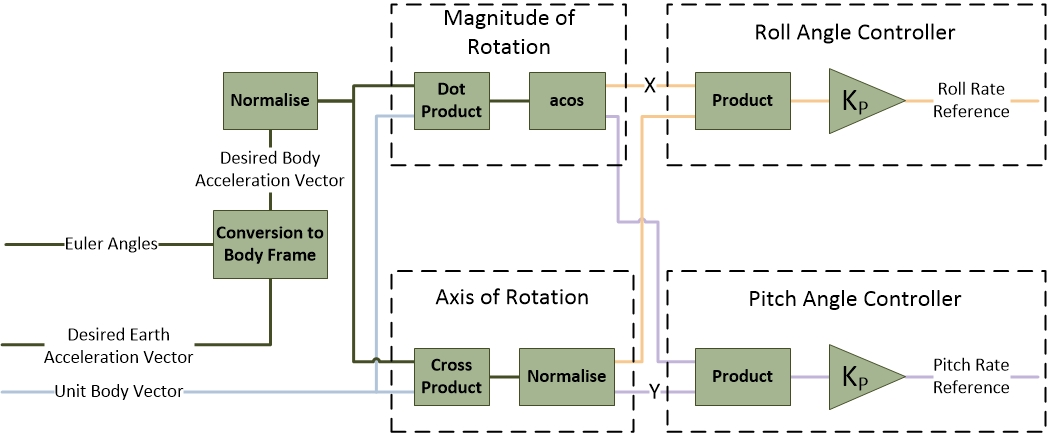
\includegraphics[height = 6.5cm]{../References/Diagrams/TiltAngleController.jpg}
	\caption{Tilt Angle Controller}
	\label{IM_TiltAngleController}
\end{figure}

\subsubsection{Method of Conversion}	
The first step to calculating the desired roll and pitch angles is to convert the earth frame set point into a body frame reference. To enable the transformation, a rotation matrix is calculated from the current Euler angles as seen in \eqref{EQ_RotationMatrix}. It is important to mention at this point that in order for accurate alignment, the desired earth acceleration vector must include a gravity component. The desired, now body, acceleration vector is normalised and then compared with a unit body vector. To remove any dependency on yaw, a unit Z body vector is created, which is perfectly aligned with the Z-Axis and thrust generation of the craft. Utilising the dot product shown in \eqref{EQ_DotProduct} the magnitude of the rotation can be calculated. Unit vectors are used, so simply taking the arc cosine of the result will produce the magnitude of rotation. The axis of rotation can subsequently be calculated by using the cross product shown in \eqref{EQ_CrossProduct} and normalising the output to remove any magnitude. Figure \ref{IM_AngleMethod} is used a visual aid for the preceding description.

\begin{equation}
\label{EQ_DotProduct}
\vec{a} \, \bigcdot \, \vec{b} = |ab|\,\cos \alpha
\end{equation}

\begin{equation}
\label{EQ_CrossProduct}
\vec{a} \, \times \, \vec{b} = \vec{c}
\end{equation}

\begin{figure}[H]
	\centering
	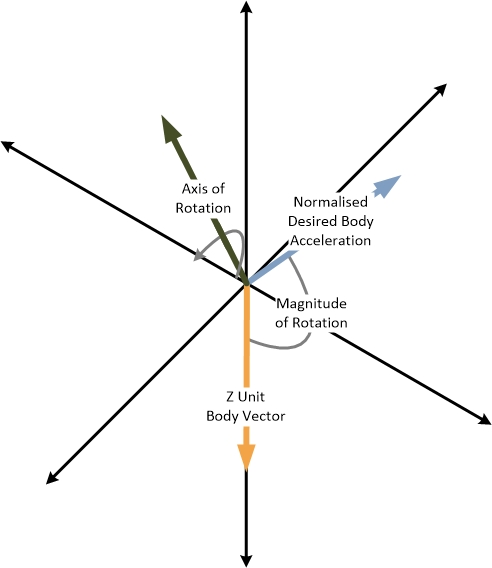
\includegraphics[height = 10cm]{../References/Diagrams/ConversionMethod.jpg}
	\caption{Conversion Technique using Dot and Cross Products}
	\label{IM_AngleMethod}
\end{figure}

\subsubsection{Roll and Pitch Angle Controllers}
The linear analysis of the tilt angle controller is done by simplifying the system as shown in Figure \ref{IM_RollAngleLoop}. The additional time required to calculate the setpoints and the rotation matrix can be considered in the design by ensuring sufficient phase margin. As mentioned in the rate controller section, the outer controllers are limited by the inner loop bandwidth. The roll and pitch angle controllers must account for this by having a slower system with less bandwidth. For practical systems, the ratio between the inner and outer loop should be in the region of $2 - 4$. The inner rate controller includes an integrator term and can handle disturbances, thus allowing for a less complex angle control law. 

\begin{figure}[H]
	\centering
	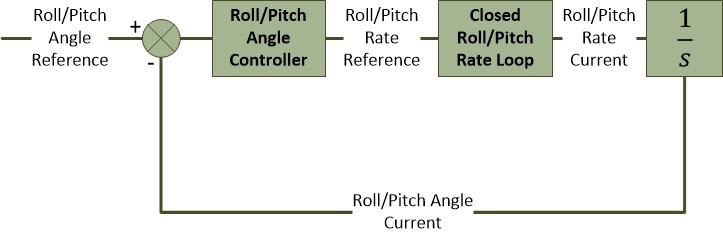
\includegraphics[height = 3.5cm]{../References/Diagrams/RollPitchAngleLoop.jpg}
	\caption{Roll and Pitch Angle Simplified Closed Loops}
	\label{IM_RollAngleLoop}
\end{figure}

The roll angle loop's frequency response is shown in the Bode plot in Figure \ref{IM_RollAngleControlBode}. Unity feedback is compared against the chosen controller. The integration between rate and position increases the phase in the lower frequencies producing sufficient phase, allowing for a simple Proportional (P) control law in the angle loop. The final phase margin is $78$\textdegree. The controller adds a bit more gain than unity feedback and increases the bandwidth while pushing the crossover frequency to $1.26$\,rad/s. There is now a ratio of $3.8$ between the inner and outer loop. From observation there is still more room for a faster system and increased bandwidth. However, the damping decreases as the system is pushed harder creating a need for more complex control law, with little gain benefit.

\begin{figure}[H]
	\centering
	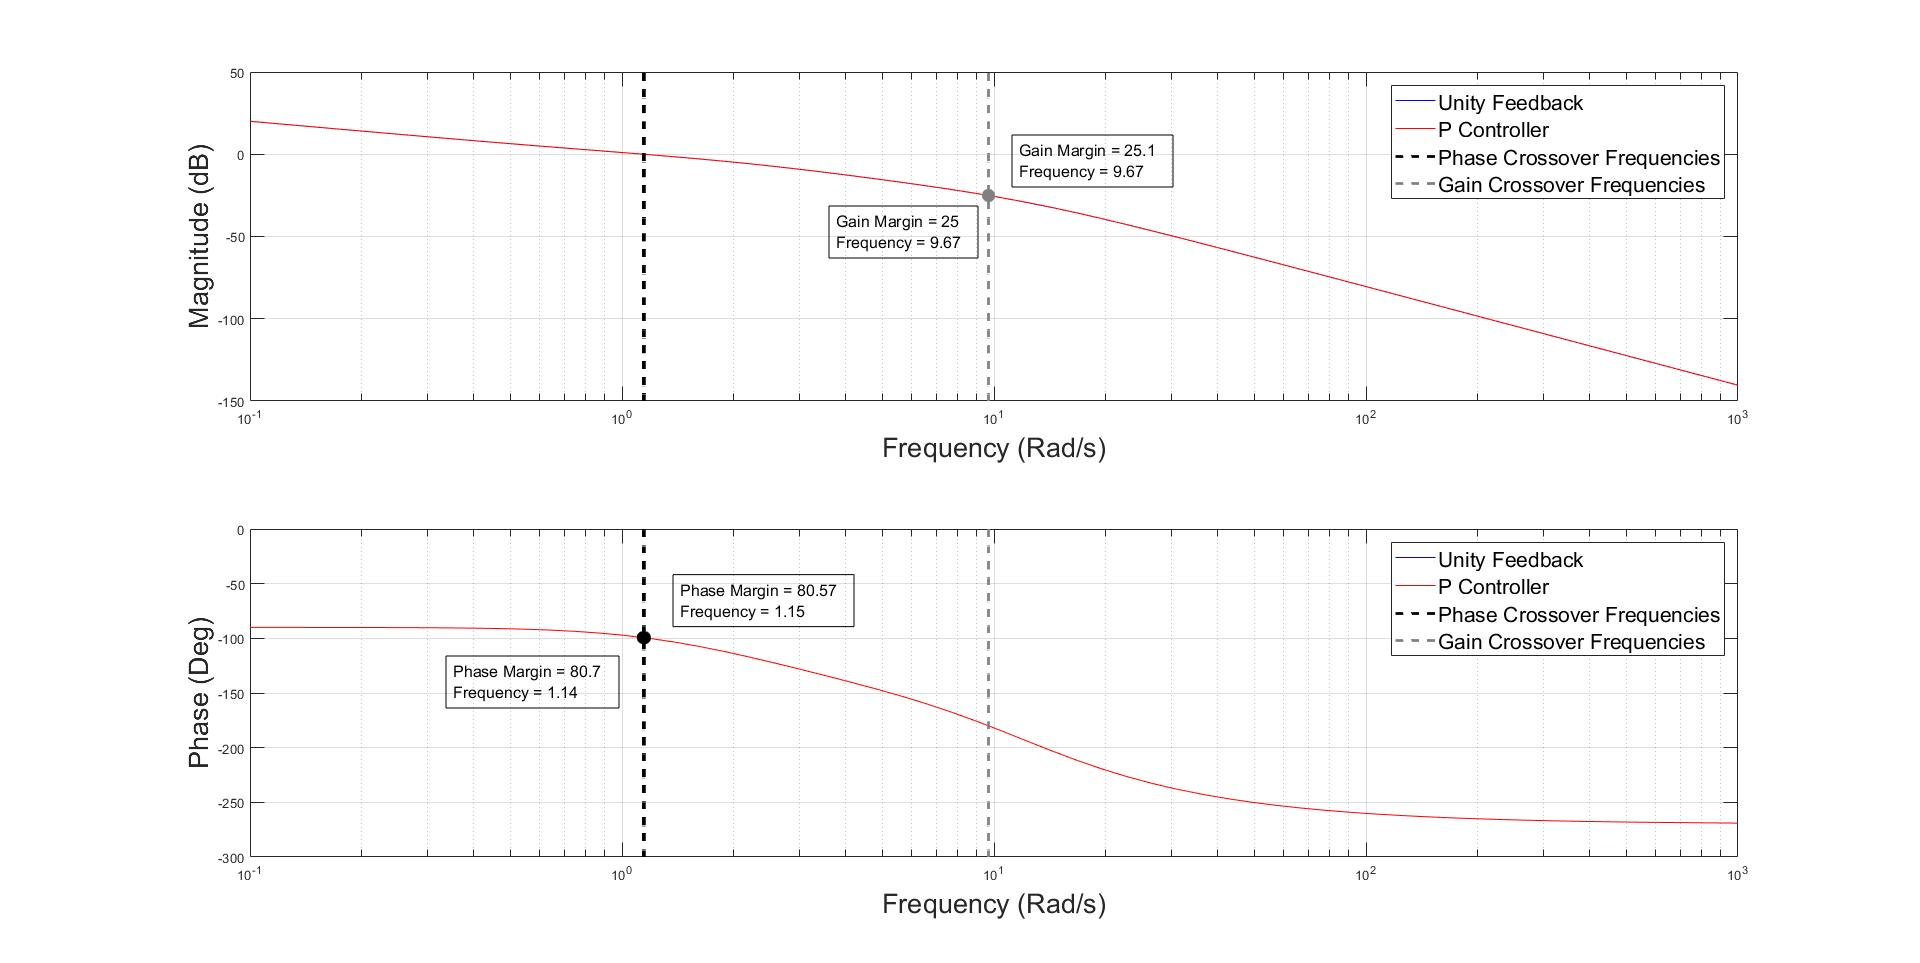
\includegraphics[height = 8cm]{../Design/Matlab/Controllers/roll_angle_bode.jpg}
	\caption{Roll Angle Controller -  Bode Plots}
	\label{IM_RollAngleControlBode}
\end{figure}

\subsubsection{Tilt Angle Controller Discussion}
The time domain response of the system is evaluated and discussed next. To draw a comparison between the roll and pitch systems their step responses are plotted together in Figure \ref{IM_RollAngleStep}. As desired, the roll and pitch angle transient responses are almost identical. The final rise time for both systems is $1.65$\,s and they both successfully have zero steady state error. The same disturbances used in the rate loop are applied to this system at $10$\,s. As shown, both systems handle the disturbance successfully. Although, as expected, the pitch system deviates less from the reference.

\begin{figure}[H]
	\centering
	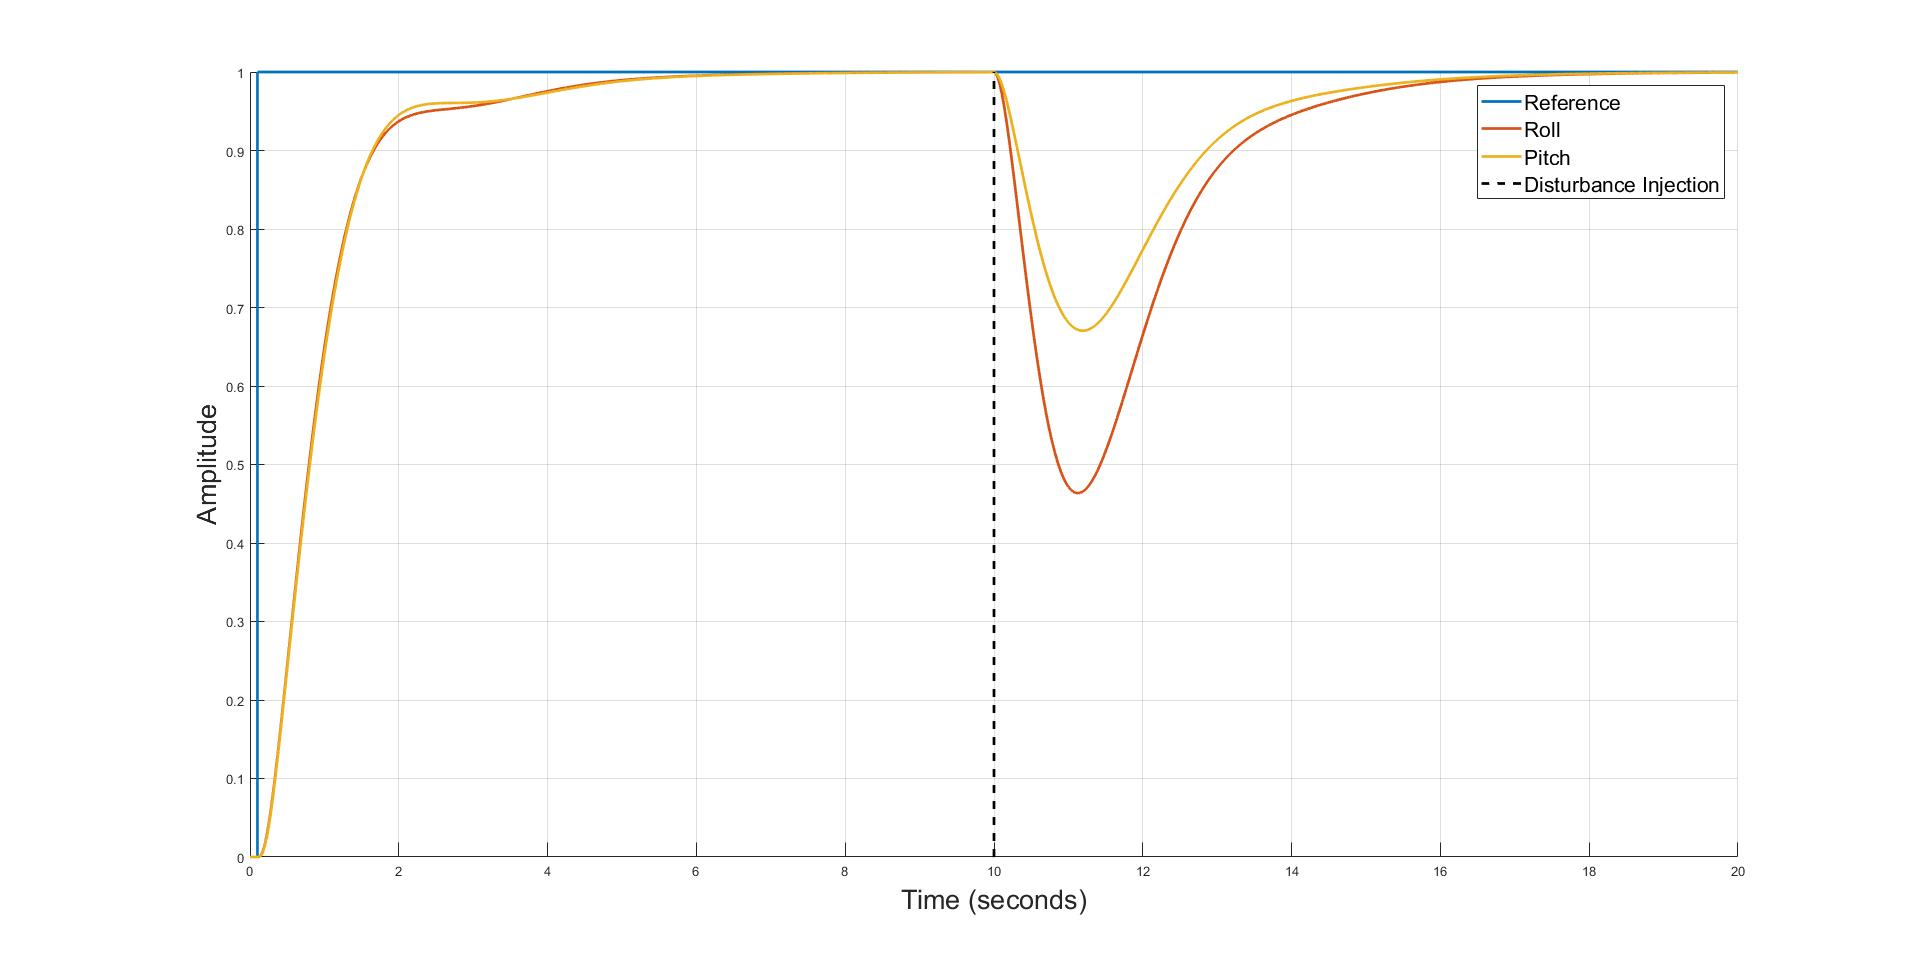
\includegraphics[height = 8cm]{../Design/Matlab/Controllers/roll_pitch_angle_step.jpg}
	\caption{Roll and Pitch Angle Controller -  Step Responses}
	\label{IM_RollAngleStep}
\end{figure}

Finally the commands sent to the motors are evaluated in Figures \ref{IM_RollAngleImpulse} and \ref{IM_PitchAngleImpulse}. The maximum thrust commanded by the pitch system is just less than $0.8$\,N. As expected the roll system commands a lower maximum of $0.57$\,N.

\begin{figure}[H]
	\centering
	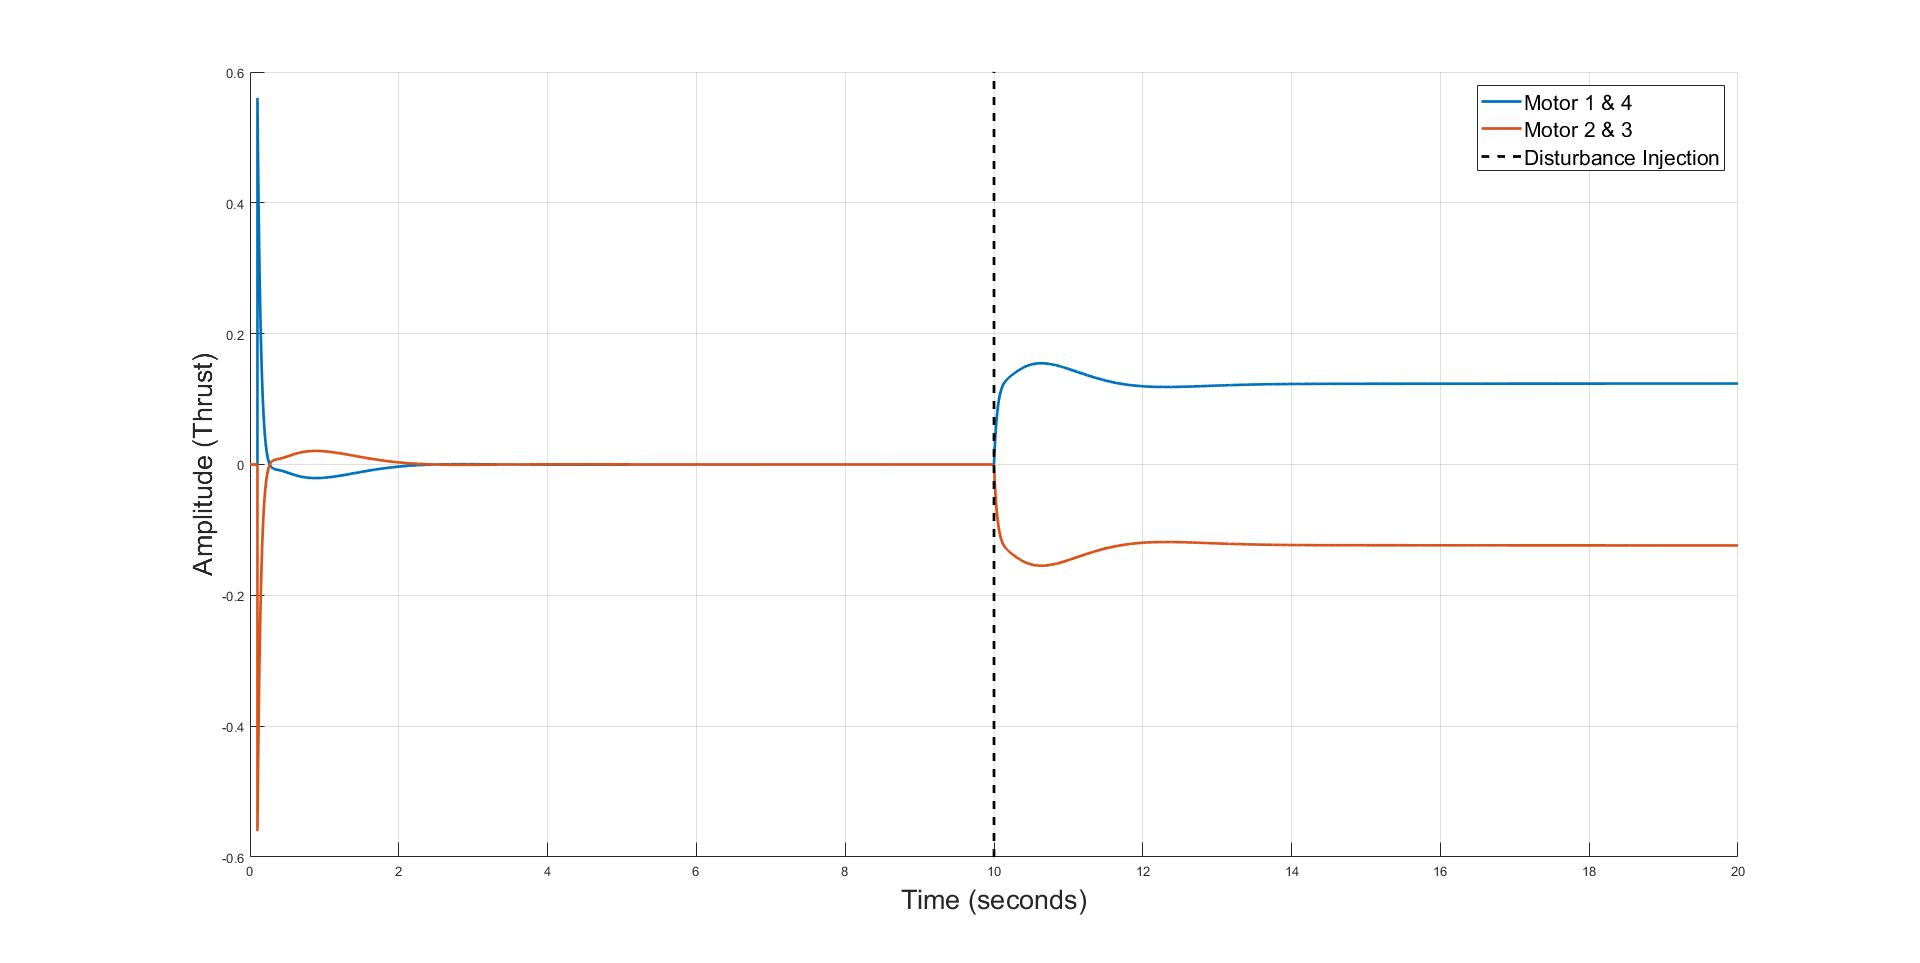
\includegraphics[height = 8cm]{../Design/Matlab/Controllers/roll_angle_impulse.jpg}
	\caption{Roll Angle Controller -  Motor Commands}
	\label{IM_RollAngleImpulse}
\end{figure}

\begin{figure}[H]
	\centering
	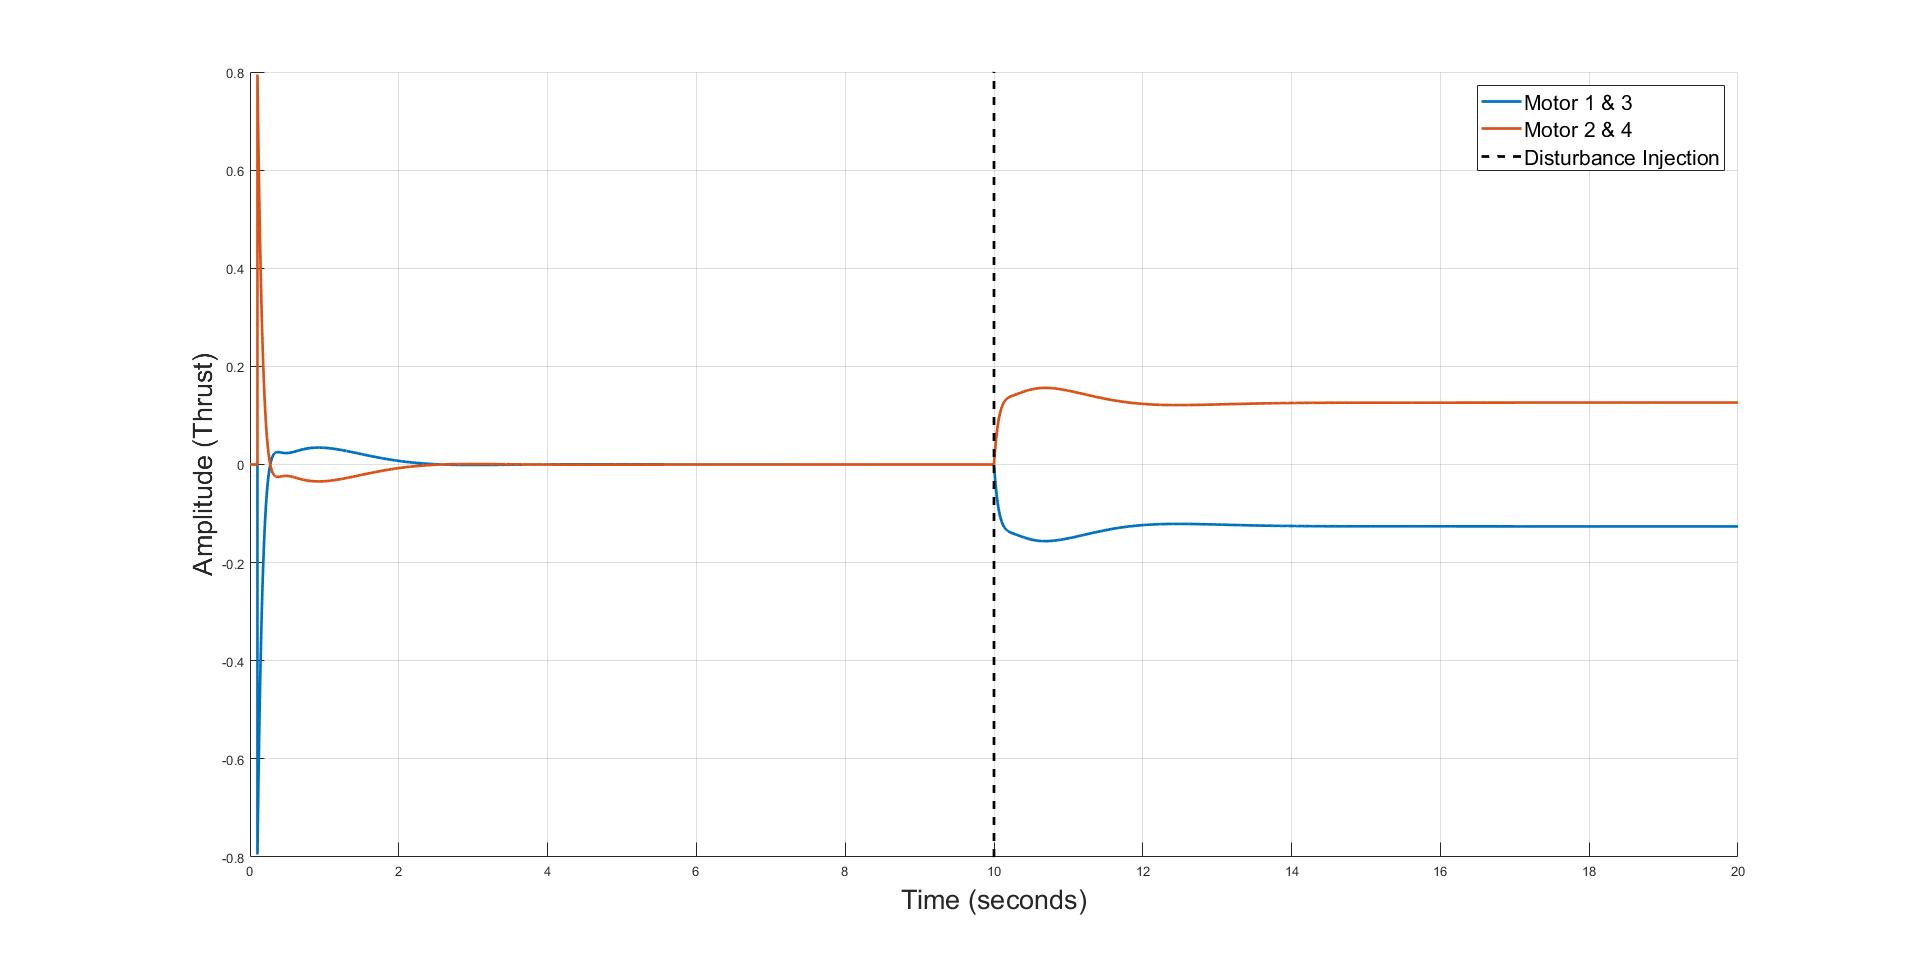
\includegraphics[height = 8cm]{../Design/Matlab/Controllers/pitch_angle_impulse.jpg}
	\caption{Pitch Angle Controller -  Motor Commands}
	\label{IM_PitchAngleImpulse}
\end{figure}

\subsection{Linear Velocity Control}
This section follows the design of the linear velocity controller. This controller is responsible for controlling the translational velocities of the craft along the North and East axis. This controller will receive a reference from the outer position loop and feed an acceleration command to the tilt angle controller. The tilt angle controller implementation successfully abstracts the angular position from the acceleration reference. However, the relationship between the pitch angle of the craft and North acceleration reference still requires a linearisation for the controller design. 

For simplification the craft is assumed to be travelling at a maintained height in a Northern direction, with zero heading. The relationship between Northern acceleration of the craft can then be defined trigonometrically by the pitch angle of the craft as seen in \eqref{EQ_LinearNorthVel}. 

\begin{eqnarray}
\ddot{N} &=& g\times \tan \theta \label{EQ_LinearNorthVel}
\end{eqnarray}

At low angles, which is expected for the craft, $\tan \theta$ can be approximated to $\theta$ allowing for the linearisation seen in \eqref{EQ_LinearNorthVel2} and \eqref{EQ_LinearNorthVel4}. The closed loop diagram can then also be simplified as shown in Figure\ref{IM_NorthVelocityLoop}.

\begin{eqnarray}
\ddot{N} &\approx& g\times \theta \label{EQ_LinearNorthVel2}\\\label{EQ_LinearNorthVel3}
\theta 	&\approx& \frac{\ddot{N}}{g} \label{EQ_LinearNorthVel4}
\end{eqnarray}

\begin{figure}[H]
	\centering
	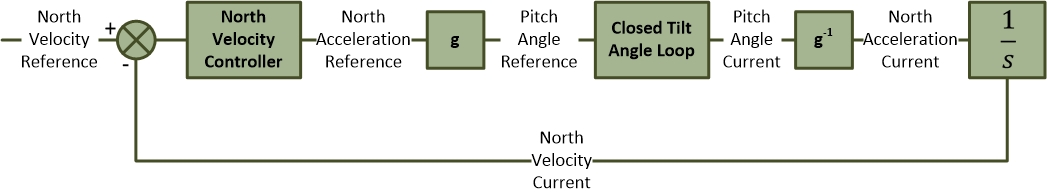
\includegraphics[height = 2.9cm]{../References/Diagrams/NorthVelocityLoop.jpg}
	\caption{North East Simplified Closed Loops}
	\label{IM_NorthVelocityLoop}
\end{figure}

The allowed bandwidth of the linear velocity controller is limited by the bandwidth of the tilt angle controller. The free integrator in the linear velocity loop will ensure that the system will track a set point with zero steady state error. However, there are expected disturbances which require more complex control than proportional control to reject. The Bode plots in Figure \ref{IM_NorthVelControlBode} assist with the design by allowing easy analysis of phase and gain in the system.

A traditional PI architecture increases the low frequency gain, however was not suitable due to the loss in phase and damping. Instead a lag compensator could be designed to limit the overshoot while enabling some disturbance rejection. The process of designing the lag compensator under went the following steps. First a proportional controller is designed to achieve the desired bandwidth, $\omega_{des}$. The zero of the compensator is then placed far enough to negate any effect on the bandwidth. The pole has been placed to optimise both limiting overshoot and enabling disturbance rejection.

As desired the P and lag controlled systems exhibit the same crossover frequency bandwidth and negligibly different high gain profiles. Both the lag compensator and the PI controller increase the low bandwidth gain at the cost of some phase. However, the phase benefits of the lag compensator compared to the PI controller can be seen clearly. The final system is designed to have a crossover frequency of $0.42$\,rad/s and a phase margin of $65$\textdegree. This bandwidth is a ratio $2.7$ slower than the slowest loop in the tilt angle controller.

\begin{figure}[H]
	\centering
	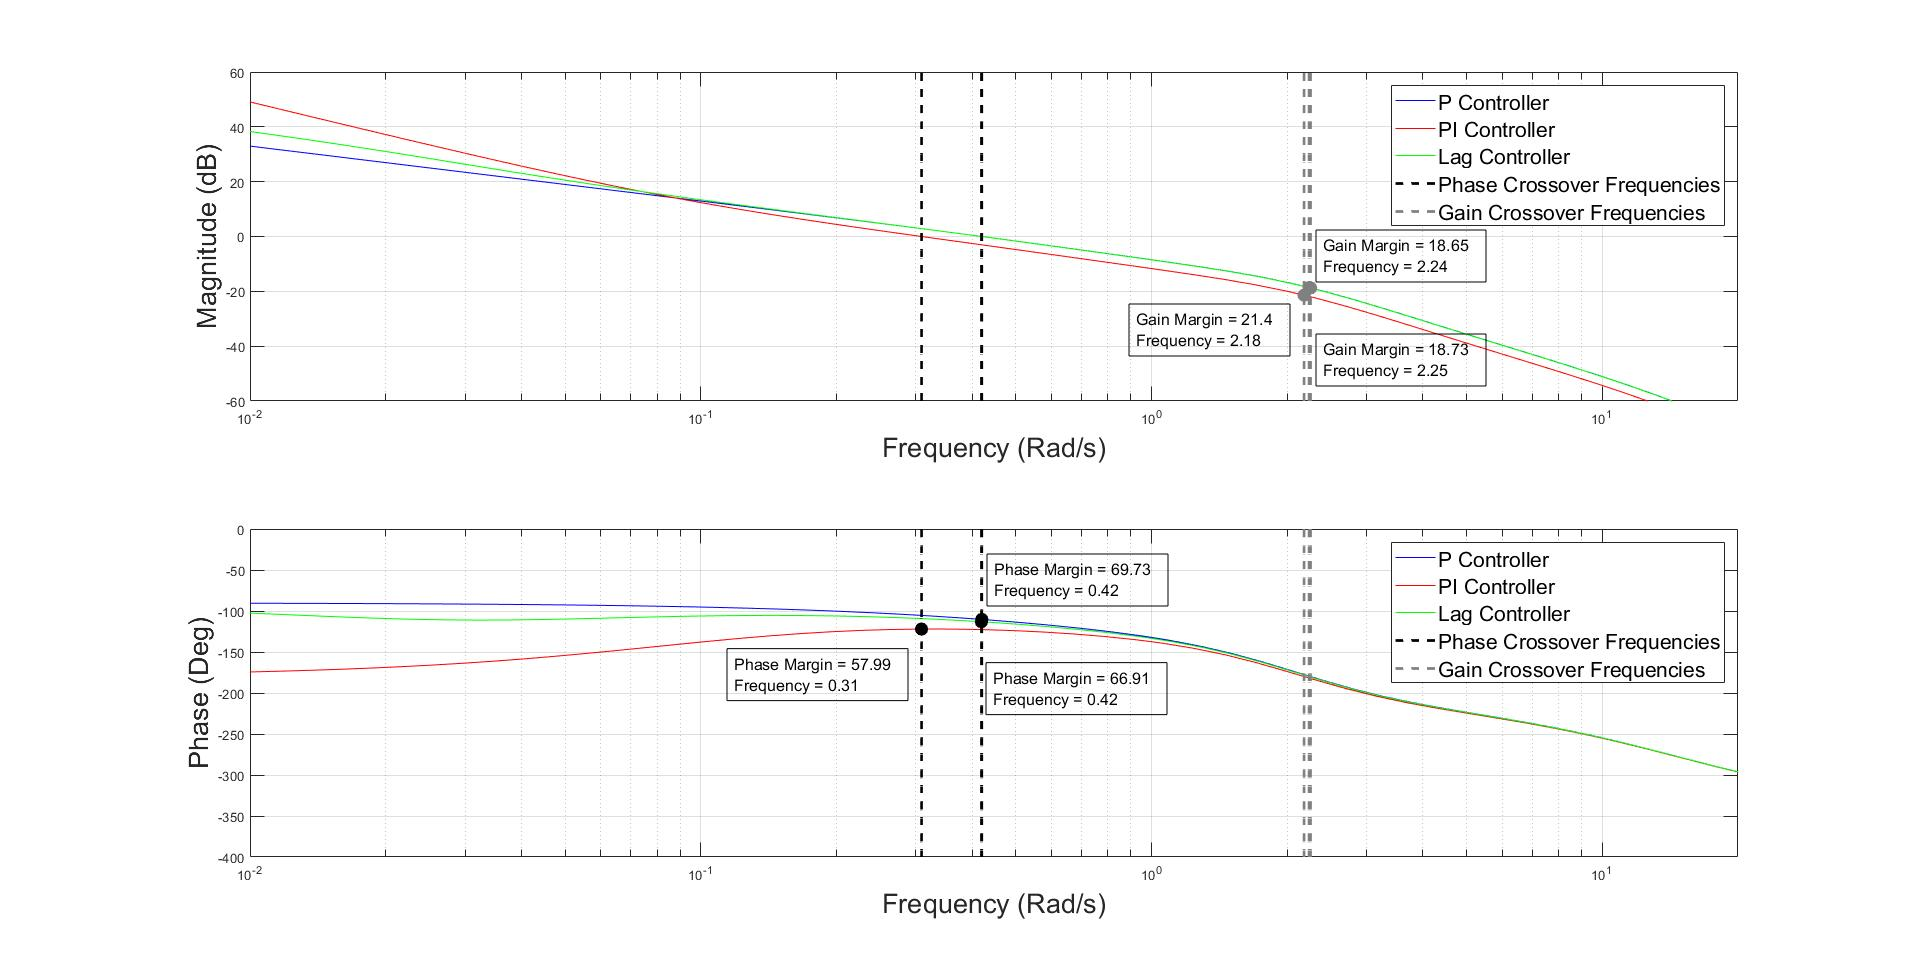
\includegraphics[height = 8cm]{../Design/Matlab/Controllers/north_velocity_bode.jpg}
	\caption{North Velocity Controller -  Bode Plots}
	\label{IM_NorthVelControlBode}
\end{figure}

The final placement of the lag compensator can be shown on the root locus in Figure \ref{IM_NorthVelControlRoot}. The compensator zero has been placed at $\dfrac{\omega_{des}}{10}$ with the pole a factor of $4$ slower.

\begin{figure}[H]
	\centering
	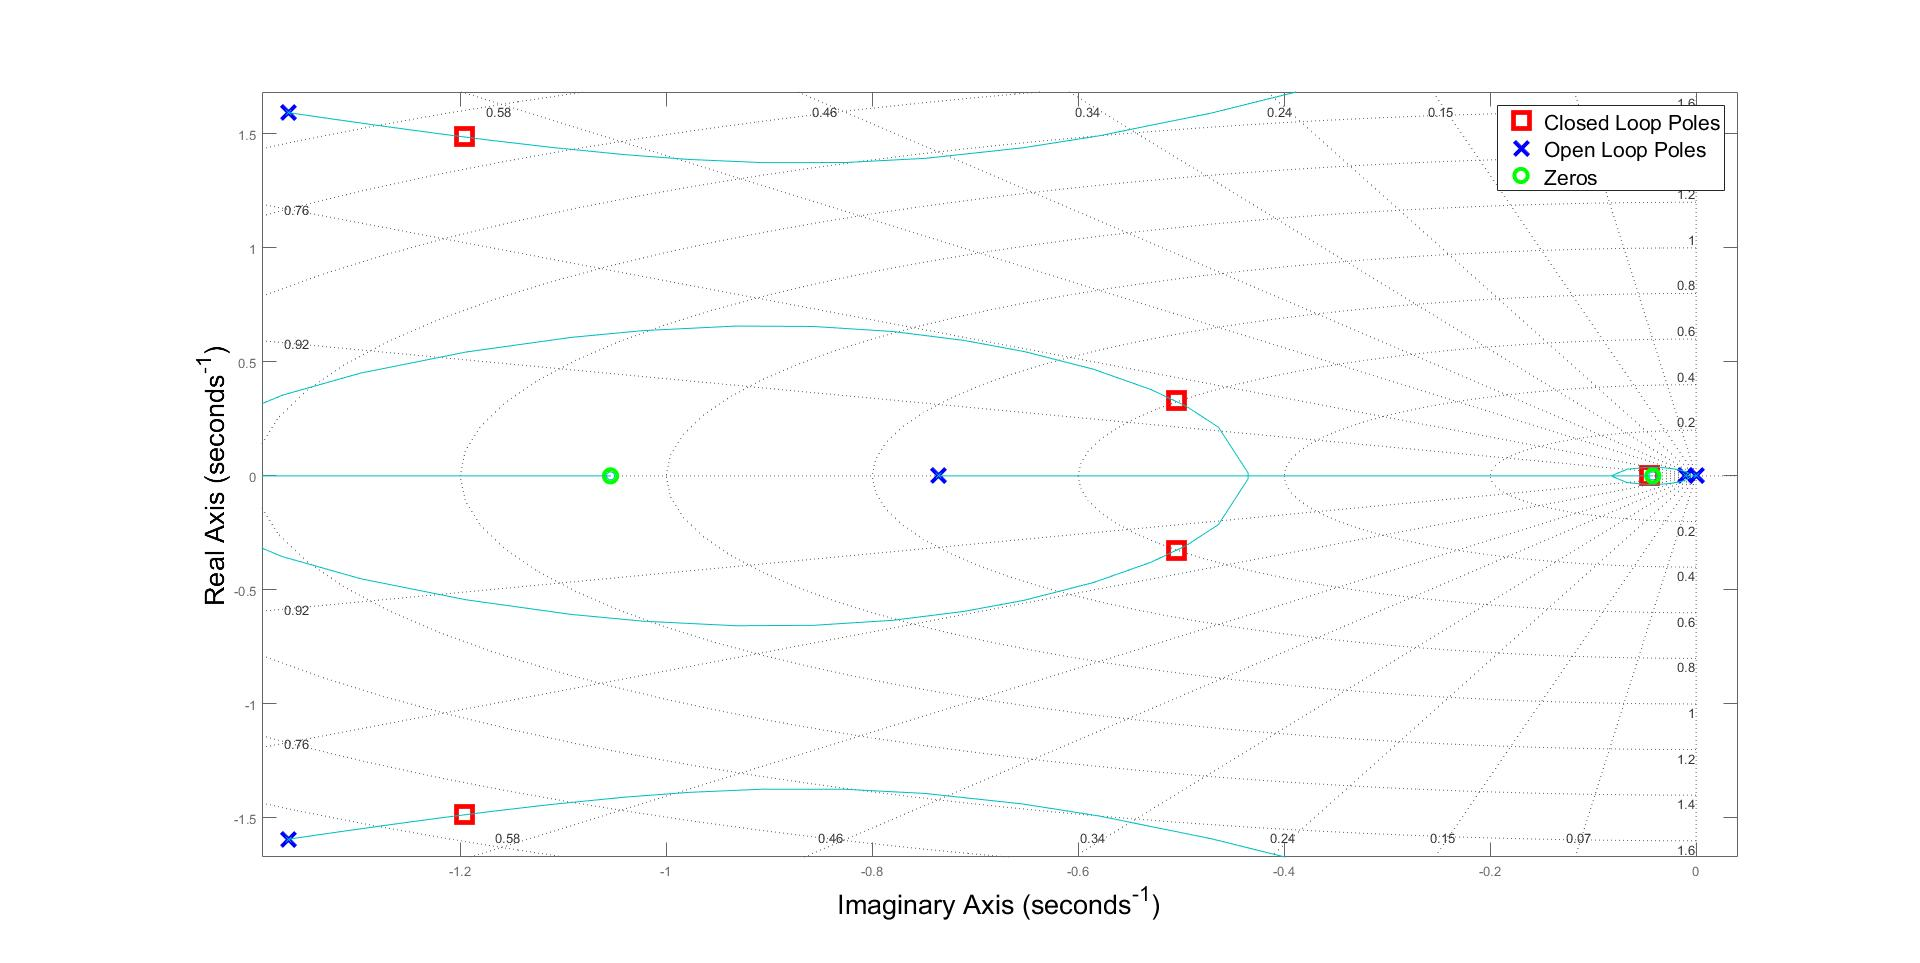
\includegraphics[height = 8cm]{../Design/Matlab/Controllers/north_velocity_root.jpg}
	\caption{North Velocity Controller -  Root Locus Plot}
	\label{IM_NorthVelControlRoot}
\end{figure}	

\subsubsection{Linear Velocity Controller Discussion}
The three controllers all exhibit a stable dynamic response, the differences in gain and phase were identified and discussed in the Bode plot. The time domain responses and differences can now be evaluated and discussed. The step response of the P, PI and lag controllers are shown in Figure \ref{IM_NorthVelControlStep}. The proportional controller has a fast transient response with a rise time of $3.3$\,s. The P controller exhibits good phase margin and shows little overshoot. The lose in phase of the PI controller presents itself as a large overshoot of $20$\%. The integrator introduces a long tail into the system and slows the transient response to a rise time of $4.9$\,s. The lag compensator has some overshoot and a very similar transient response to the P controller.

\begin{figure}[H]
	\centering
	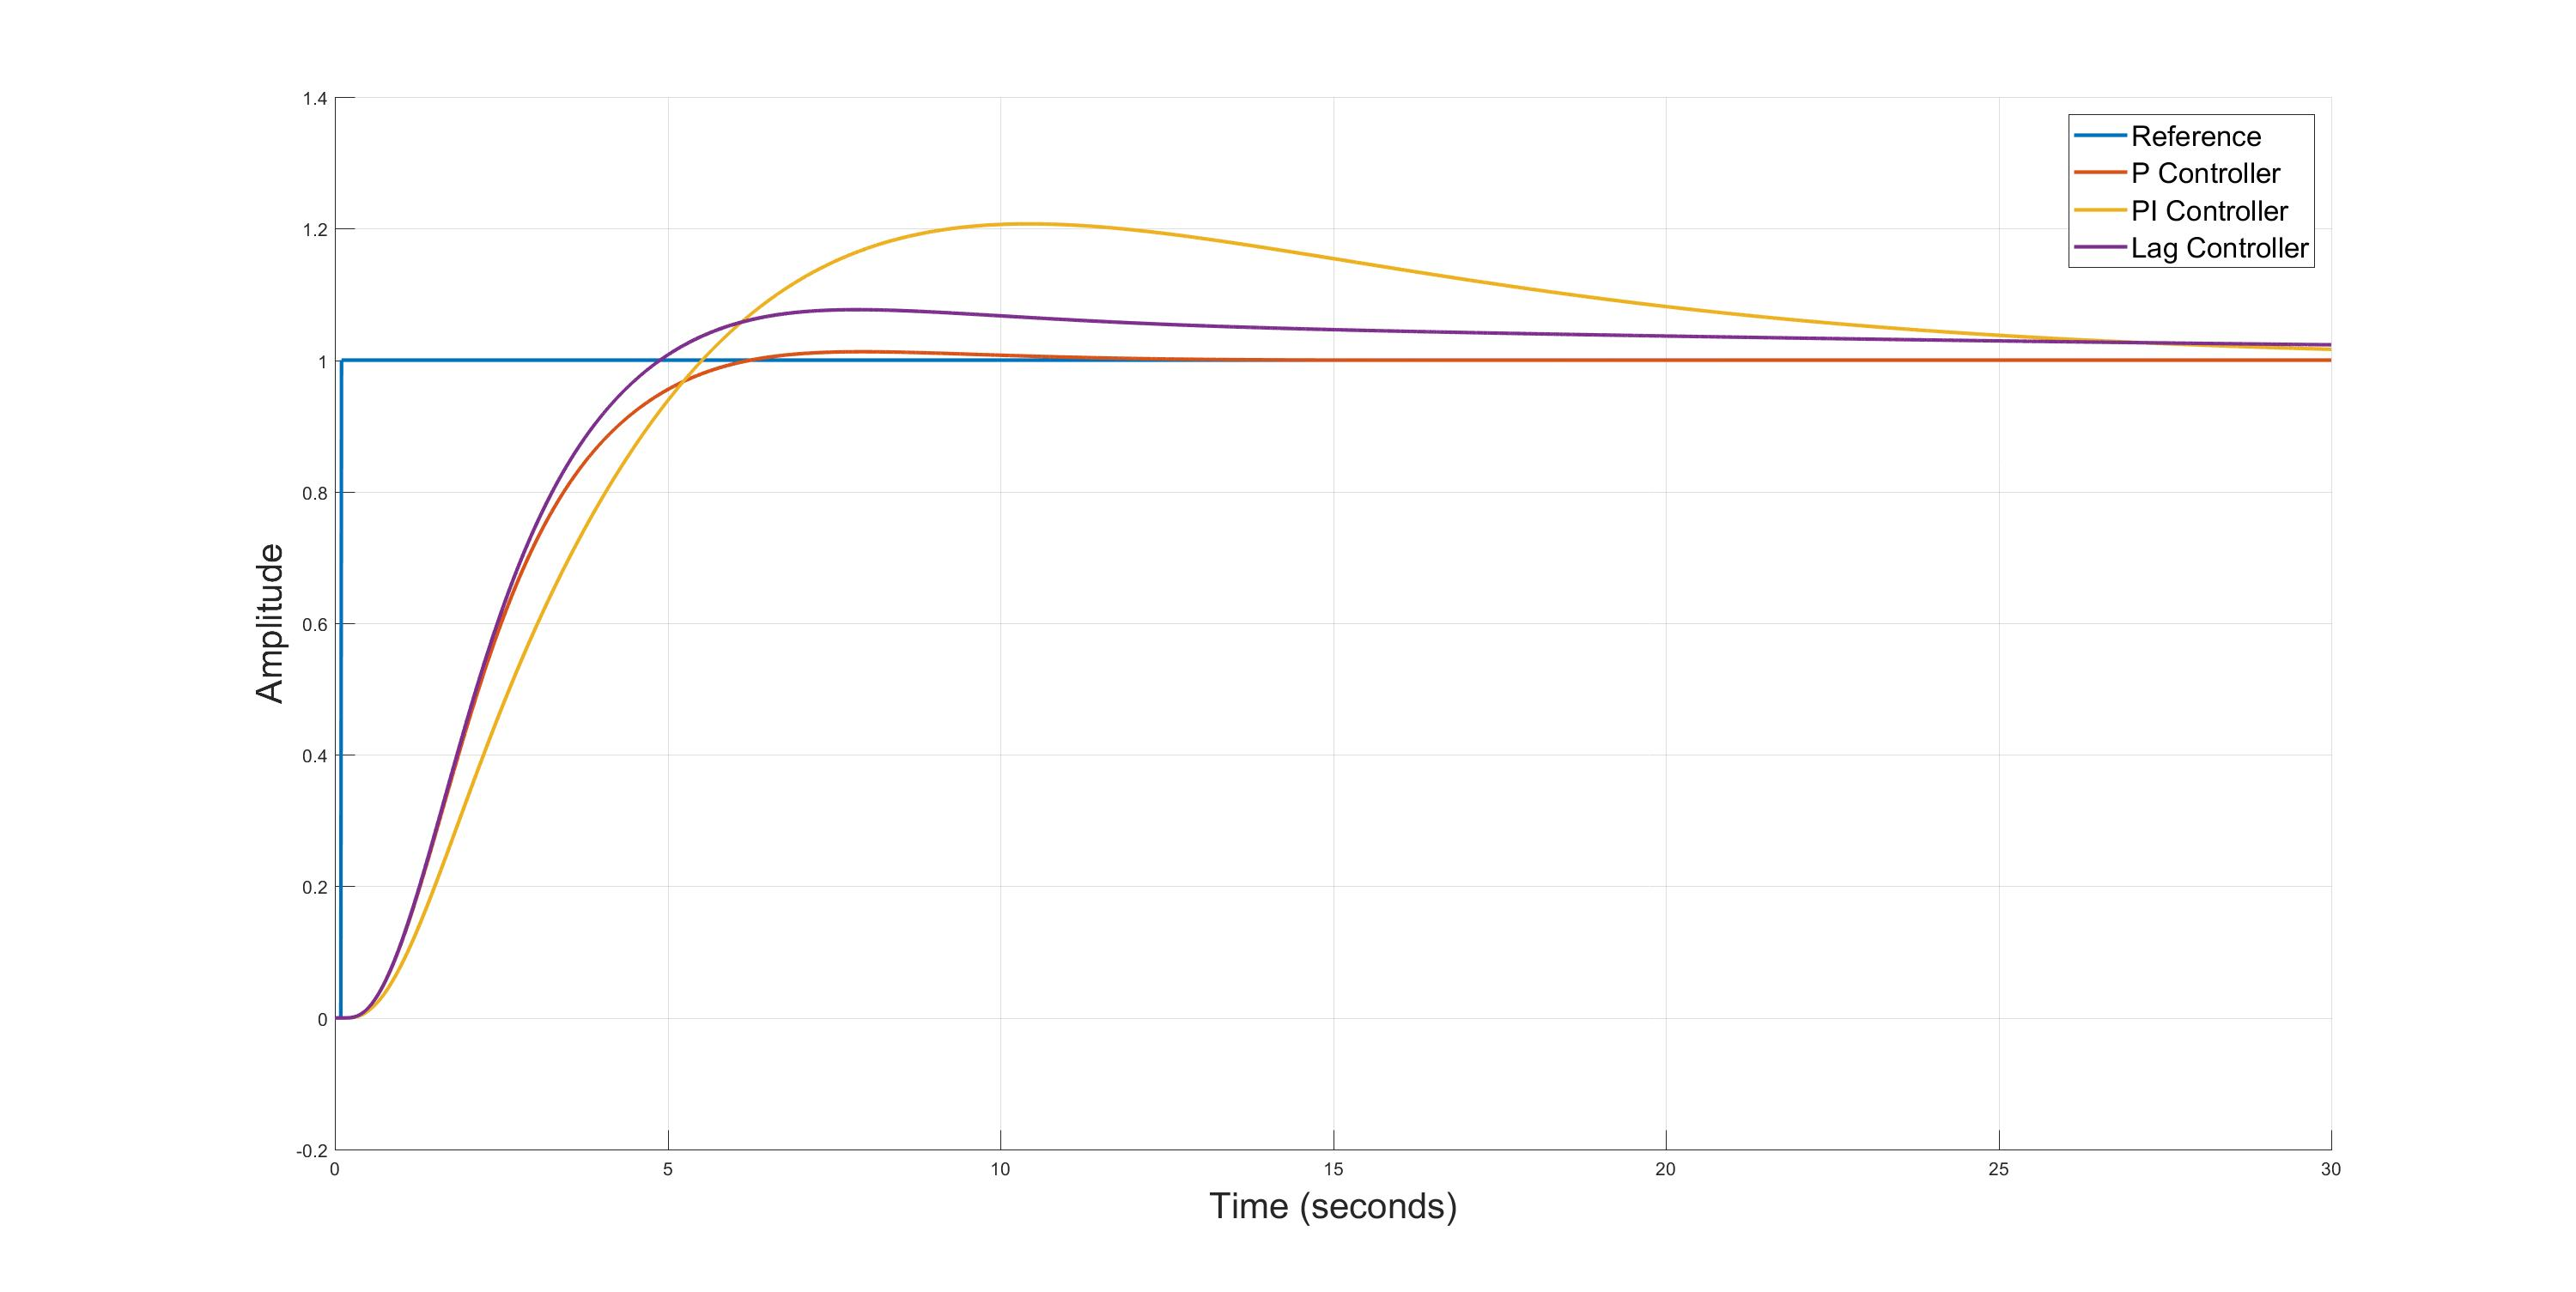
\includegraphics[height = 8cm]{../Design/Matlab/Controllers/north_velocity_step.jpg}
	\caption{North Velocity Controller -  Step Responses}
	\label{IM_NorthVelControlStep}
\end{figure}	

The benefit of the lag compensator over th P controller can be seen when a disturbance is introduced into the system. Figure \ref{IM_NorthVelControlDistStep} is used to show the effect of a constant disturbance in the system by adding an external force at $30$\,s. The P controller is unable to reject the disturbance. The increased low bandwidth gain of the lag compensator manages to reduce the disturbance and as expected the PI controller successfully rejects the disturbance completely.

\begin{figure}[H]
	\centering
	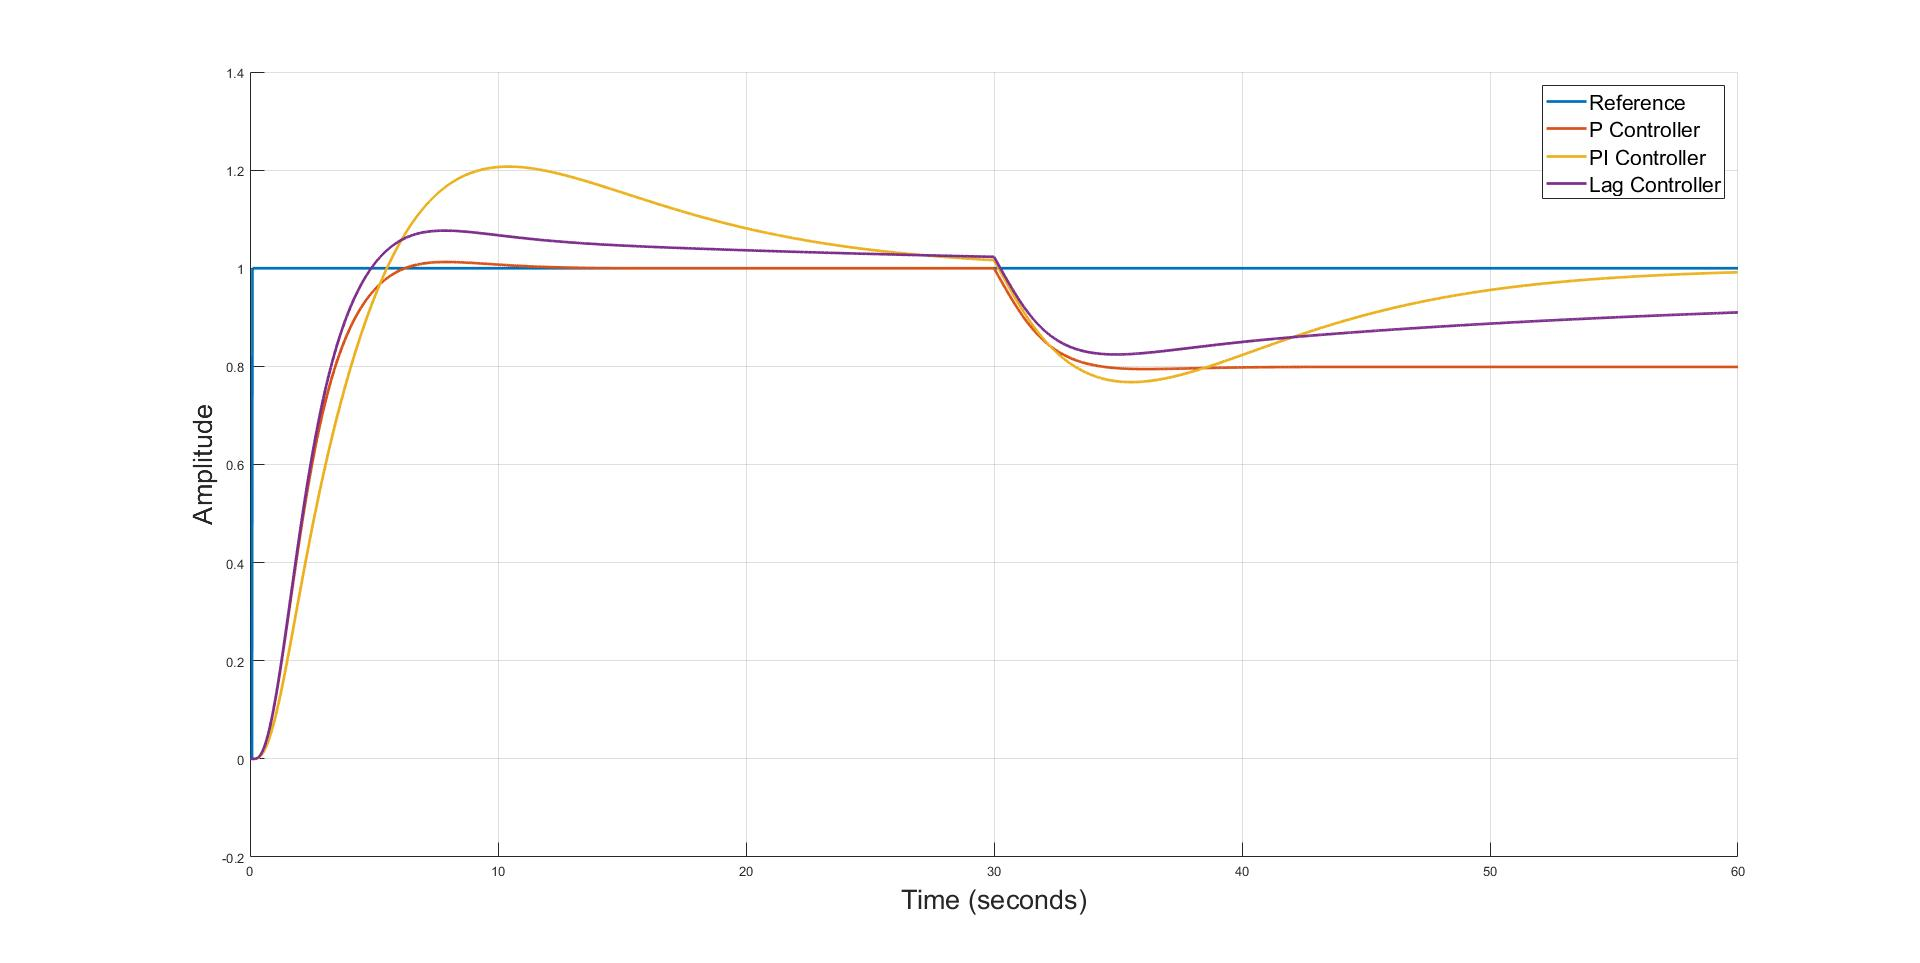
\includegraphics[height = 8cm]{../Design/Matlab/Controllers/north_velocity_stepd.jpg}
	\caption{North Velocity Controller -  Step Responses With a Disturbance}
	\label{IM_NorthVelControlDistStep}
\end{figure}	

\subsection{Global Position Tracking Control}
The position controller is the most outer loop of the horizontal controller and will be fed a reference from a waypoint generator or some other, high level flight strategy. There is sufficient disturbance rejection in the inner loops allowing the position controller to use a simple proportional controller. The final bandwidth should utilise the full potential of the inner loop velocity system. The craft should approach a set point steadily and with little overshoot, the final system should thus be well damped.

The Bode plot in Figure \ref{IM_NorthPosControlBode} is used for the design as it easily shows the phase and gain margins of the system. The plant is on the edge of stability and is compared with a controlled system utilising a P controller. The proportional gain is adjusted until there is sufficient phase margin of $69$\textdegree and gain margin of $17$\,dB. The final cross over frequency is $0.16$\,rad/s, creating a ratio of $2.6$ between the inner and outer loop.

\begin{figure}[H]
	\centering
	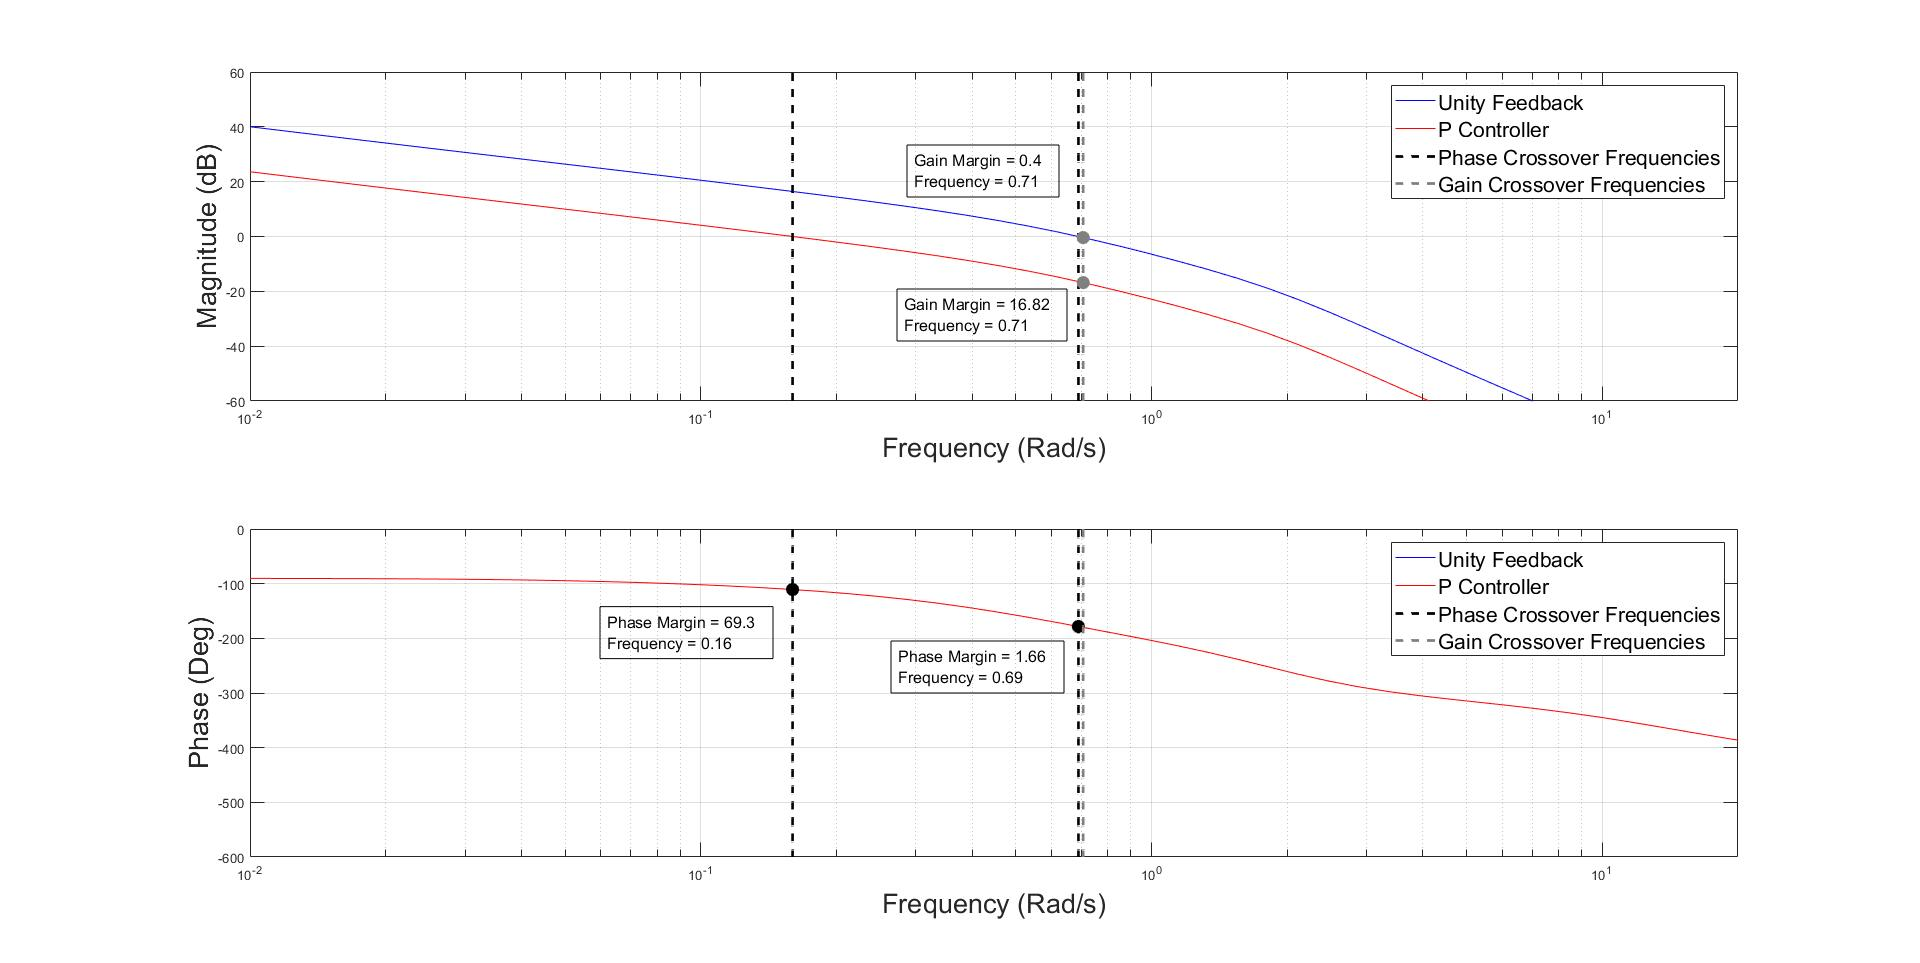
\includegraphics[height = 8cm]{../Design/Matlab/Controllers/north_position_bode.jpg}
	\caption{North Position Controller -  Bode Plots}
	\label{IM_NorthPosControlBode}
\end{figure}

\subsubsection{Position Controller Discussion}
The proportional gain increase stability in the system and reduces the crossover frequency. Figure \ref{IM_NorthPosControlStep} represents the step response of the system. The system is shown to be well damped with no oscillatory motion in the response. 

\begin{figure}[H]
	\centering
	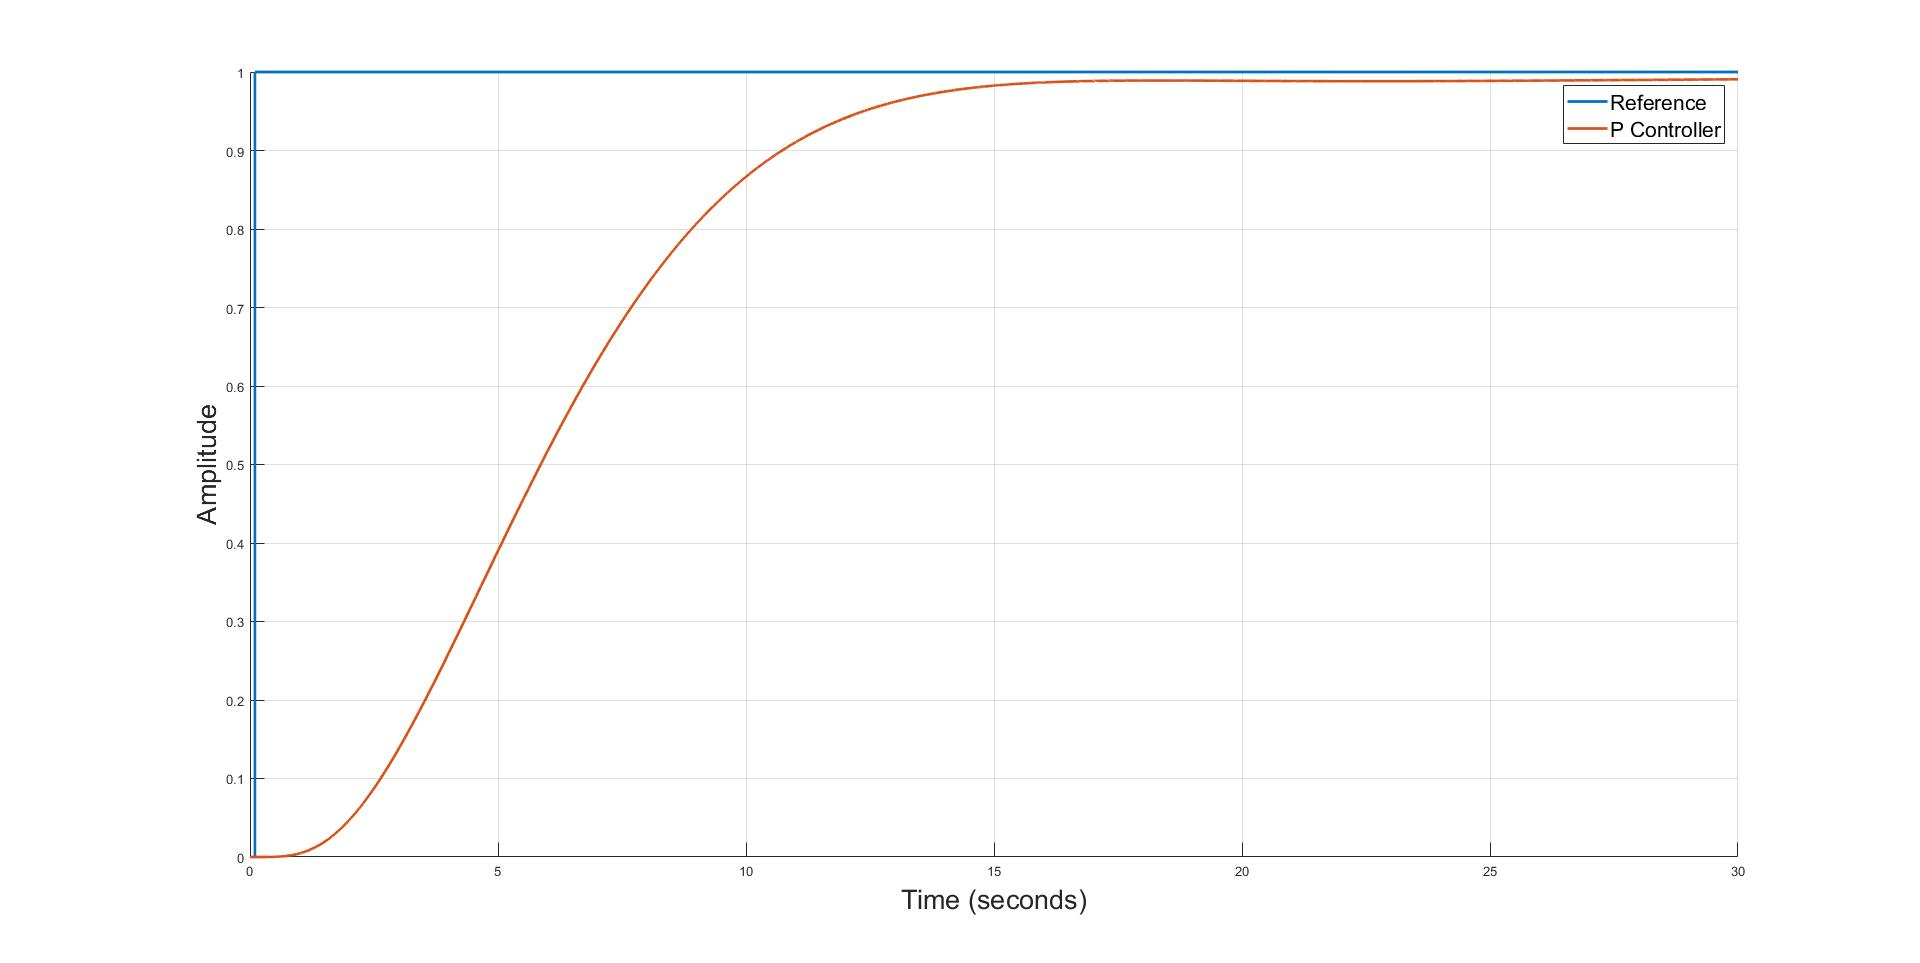
\includegraphics[height = 8cm]{../Design/Matlab/Controllers/north_position_step.jpg}
	\caption{North Position Controller -  Step Response}
	\label{IM_NorthPosControlStep}
\end{figure}

The position controller could be commanded with large step values. To prohibit commanding large velocity values a limiter is used. Figure \ref{IM_NorthPosControlLargeStep} is used to show the effect the saturation has for a large step input command. 

\begin{figure}[H]
	\centering
	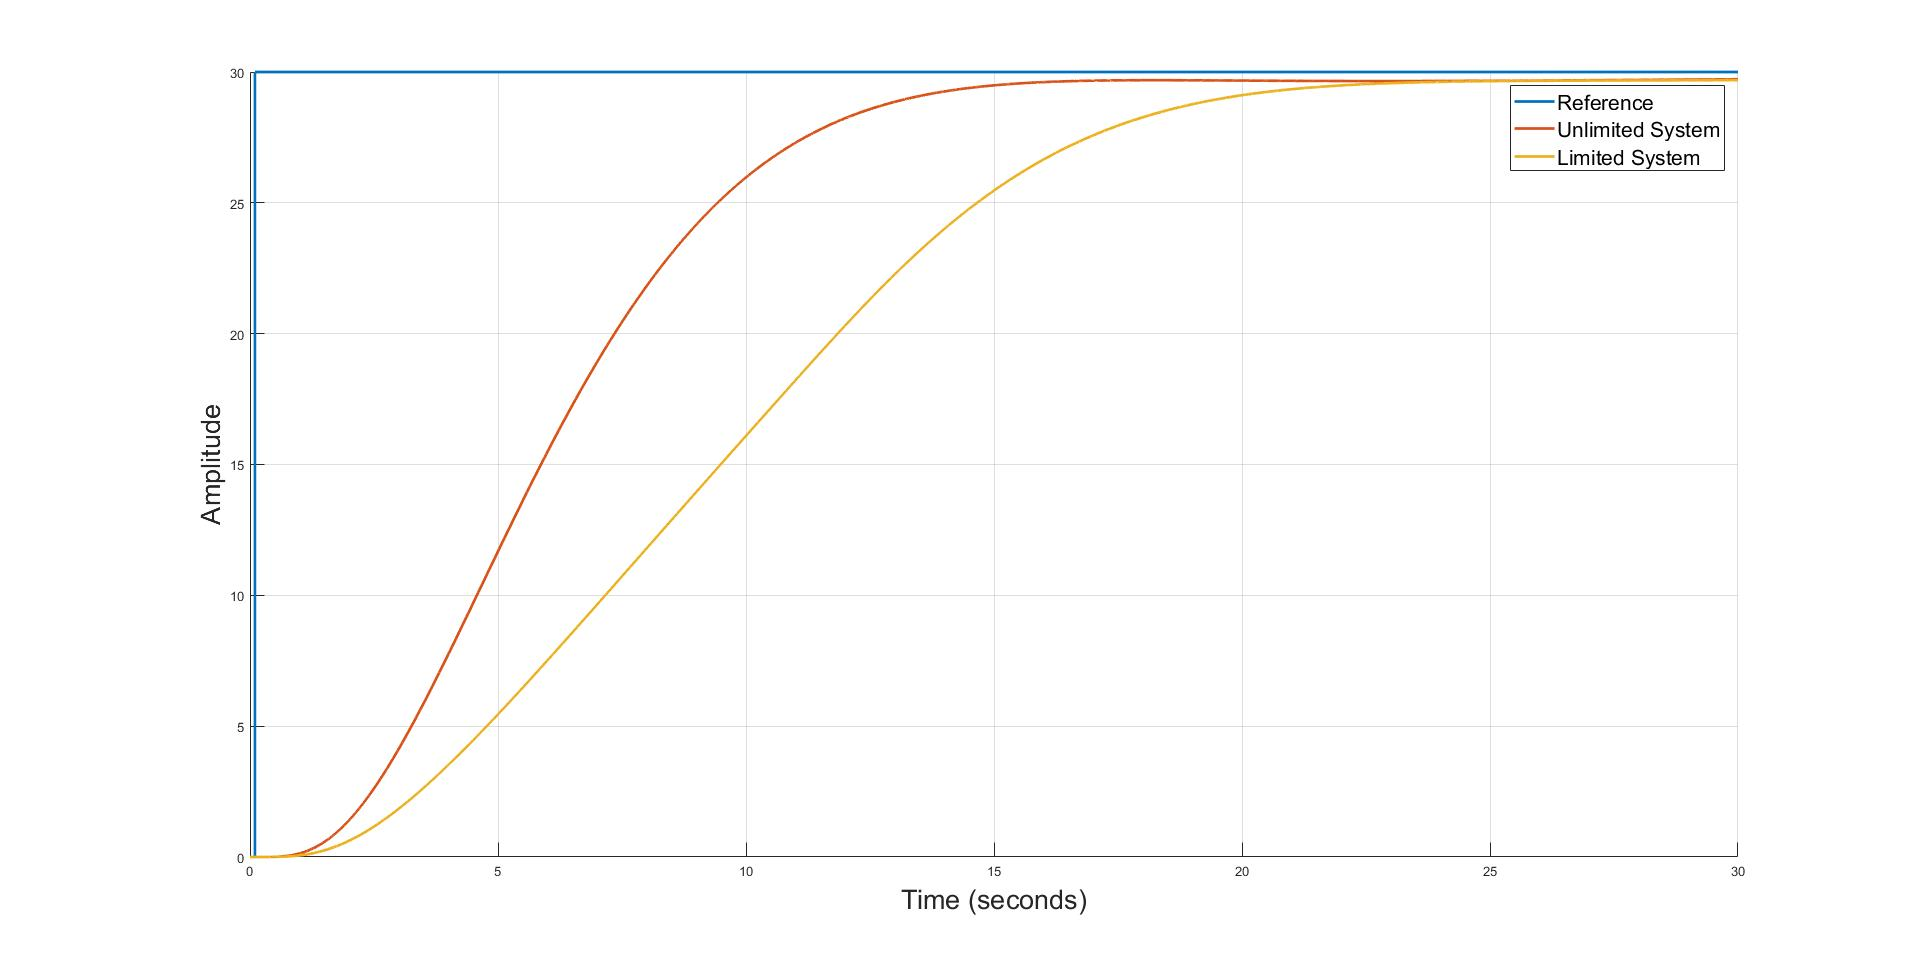
\includegraphics[height = 8cm]{../Design/Matlab/Controllers/north_pos_limit_step.jpg}
	\caption{North Position Controller -  Large Step Response With and Without a Limiter}
	\label{IM_NorthPosControlLargeStep}
\end{figure}


\end{document}   